
\documentclass[11pt]{article}
\usepackage[a4paper,margin=0.85in]{geometry}
\usepackage{amsmath,amssymb}
\usepackage{graphicx}
\usepackage{booktabs}
\usepackage{longtable}
\usepackage{array}
\usepackage{float}
\usepackage{xcolor}
\usepackage{hyperref}
\usepackage{listings}
\usepackage{fancyhdr}
\usepackage{caption}
\usepackage{microtype}
\hypersetup{colorlinks=true,linkcolor=blue,urlcolor=blue}
\pagestyle{fancy}
\fancyhf{}
\lhead{Crypto regime-change detection}
\rhead{L\'opez de Prado Ch. 17 inspired}
\cfoot{\thepage}
\setlength{\headheight}{14pt}
\setlength{\parskip}{0.55em}
\setlength{\parindent}{0pt}
\definecolor{boxgray}{RGB}{245,245,245}
\lstset{basicstyle=\ttfamily\footnotesize,breaklines=true,backgroundcolor=\color{boxgray},frame=single,columns=fullflexible}

\title{\Huge Detecting Structural Breaks in Crypto Markets\\[0.25em]
\Large A beginner-friendly empirical report inspired by Chapter 17 of \emph{Advances in Financial Machine Learning}}
\author{Prepared from Binance daily OHLC market data}
\date{Generated on 2026-05-19}

\begin{document}
\maketitle

\begin{center}
\fbox{\begin{minipage}{0.92\textwidth}
\textbf{What this report does.} We take real historical crypto price data for BTC, ETH, ETC, SOL, and HYPE and apply the structural-break diagnostics discussed in Chapter 17: recursive-residual CUSUM, Chu-Stinchcombe-White CUSUM, Chow-type Dickey-Fuller, SADF, QADF, a conditional-tail ADF summary, and sub/super-martingale trend tests. The goal is educational: show how the tests behave, how to interpret the plots, and why one should treat detected regimes as research features rather than automatic trading signals.
\end{minipage}}
\end{center}

\tableofcontents
\newpage

\section{The intuition: what is a structural break?}

A \textbf{structural break} is a change in the data-generating mechanism. In markets this often means that a process that looked stable, noisy, or mean-reverting starts behaving like a momentum process, an explosive bubble, or a fast collapse. Chapter 17 motivates these breaks as valuable because many market participants adapt slowly, and their delayed reaction can create unusually good risk/reward opportunities.

The tests in this report are not ``crash predictors''. They are numerical diagnostics. A strong reading says: \emph{something about the recent price path is statistically unusual under the reference model}. That unusual behavior may be a bubble, a burst, a volatility shock, a liquidity episode, a listing effect, a leverage unwind, or simply a noisy false alarm.

\section{Data}

\subsection{Sources and sampling}

The raw source data are Binance daily OHLCV klines downloaded through the Binance API. For each asset, the report uses the largest available Binance spot USDT history when spot is available: BTCUSDT, ETHUSDT, ETCUSDT, and SOLUSDT. HYPEUSDT is not available on Binance spot in the API check used for this report, so HYPE falls back to Binance USD-M futures daily klines. All diagnostics below are computed on daily closes; there is no weekly resampling.

\begin{figure}[H]
\centering
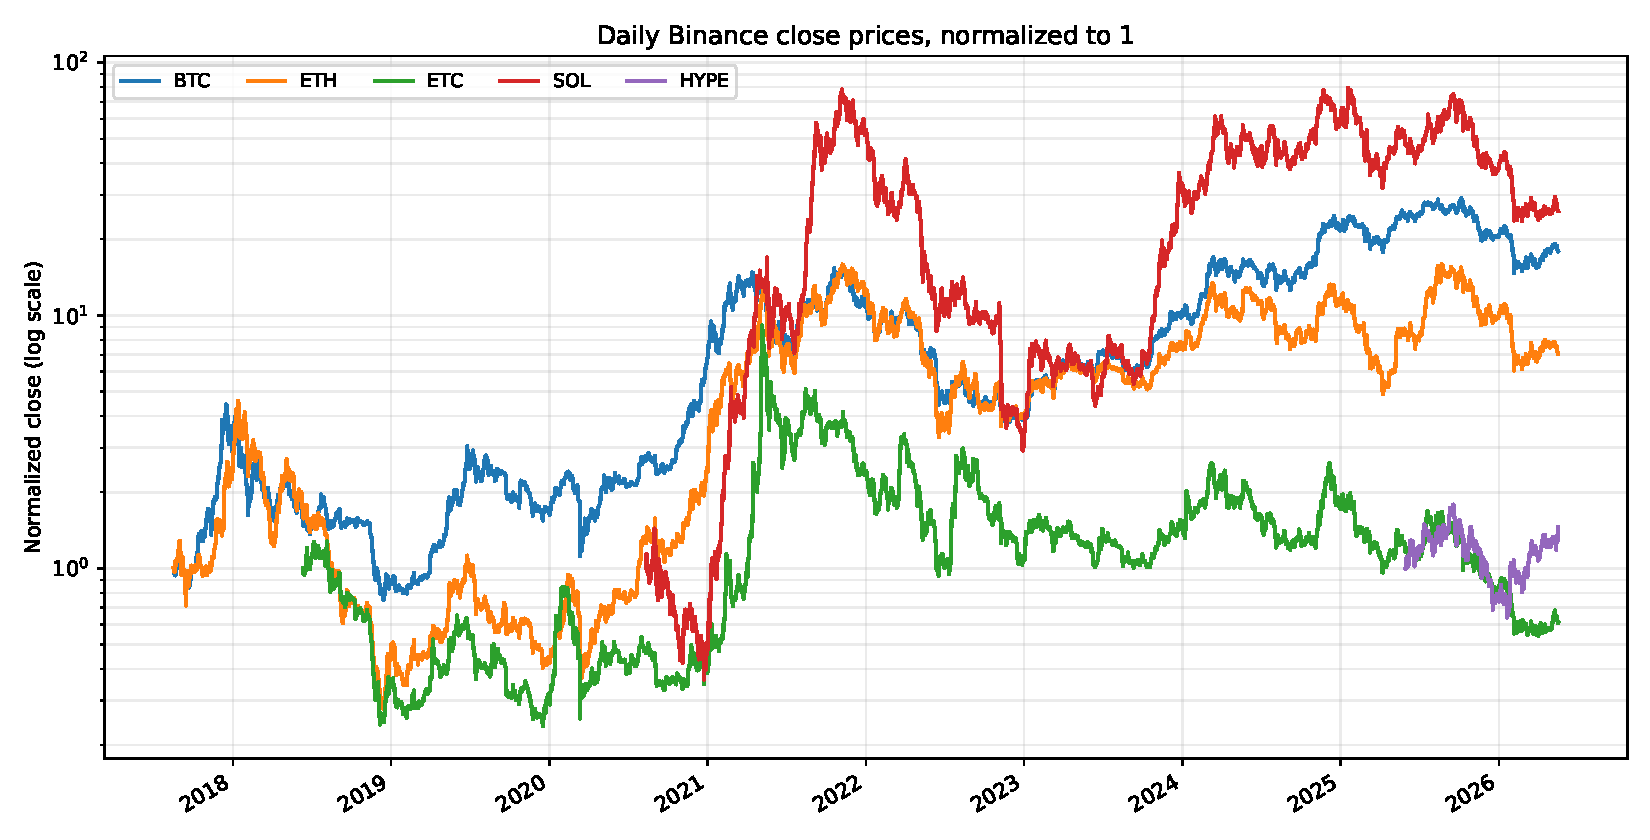
\includegraphics[width=0.98\textwidth]{regime_chapter_figs/fig01_normalized_prices.pdf}
\caption{Downloaded daily close prices, normalized to 1 at each asset's first available row. A log scale is used because crypto prices can move by orders of magnitude.}
\end{figure}

\begin{table}[H]
\centering
\scriptsize
\setlength{\tabcolsep}{3pt}
\resizebox{\textwidth}{!}{%
\begin{tabular}{@{}llccrcrrcrcccr@{}}
\toprule
Asset & Source & Raw start & Raw end & Raw rows & Clock & Test rows & $\tau$ & SDFC candidate & SDFC $t$ & Max SADF & Max CSW & Max SMT & Runs \\
\midrule
BTC & Binance spot & 2017-08-17 & 2026-05-18 & 3197 & daily close & 3197 & 480 & 2018-12-16 & 1.51 & 2021-01-08 & 2020-03-12 & 2025-10-09 & 15 \\
ETH & Binance spot & 2017-08-17 & 2026-05-18 & 3197 & daily close & 3197 & 480 & 2020-03-13 & 0.99 & 2021-05-11 & 2020-03-12 & 2021-12-02 & 24 \\
ETC & Binance spot & 2018-06-12 & 2026-05-18 & 2898 & daily close & 2898 & 435 & none (negative t) & -0.19 & 2021-05-06 & 2020-03-12 & 2021-11-03 & 8 \\
SOL & Binance spot & 2020-08-11 & 2026-05-18 & 2107 & daily close & 2107 & 317 & 2022-12-30 & 0.62 & 2023-12-25 & 2022-11-09 & 2023-01-12 & 9 \\
HYPE & Binance USD-M futures & 2025-05-30 & 2026-05-18 & 354 & daily close & 354 & 60 & 2026-01-21 & 1.44 & 2025-12-18 & 2026-01-28 & 2025-12-28 & 6 \\
\bottomrule
\end{tabular}}
\caption{Daily Binance data and headline diagnostic results. $\tau$ is the minimum daily window length used in recursive tests. ``Runs'' counts consensus alert runs, where at least two diagnostic families were simultaneously active. SDFC dates are exploratory candidates only: none of the SDFC $t$-statistics in this run clears conventional sup-DF-style critical values, and negative SDFC $t$-statistics are shown as no explosive SDFC break.}
\end{table}

The Binance API check was run on 2026-05-19 and kept candles through the last fully closed UTC day, 2026-05-18. HYPEUSDT spot returned ``Invalid symbol,'' while HYPEUSDT USD-M futures was trading, which triggered the futures fallback.

\section{The test families}

\subsection{CUSUM tests}

CUSUM means \emph{cumulative sum}. The idea is simple: if small forecast errors keep accumulating in the same direction, the model may no longer describe the market.

\textbf{Brown-Durbin-Evans recursive-residual CUSUM.} In its general form, we model
\[
    y_t = \beta_t' x_t + \varepsilon_t,
\]
fit recursively, compute one-step-ahead recursive residuals, and accumulate them. In this demonstration we only have one price series, so we use a simple trend feature vector $x_t=(1,t)$. In production, $x_t$ should be the actual forecasting feature vector used by the model.

\textbf{Chu-Stinchcombe-White CUSUM on levels.} This test asks whether log price $y_t$ has moved too far from an earlier reference level $y_n$ relative to realized volatility:
\[
    S_{n,t} = \frac{y_t-y_n}{\hat\sigma_t\sqrt{t-n}},
    \qquad
    \hat\sigma_t^2 = \frac{1}{t-1}\sum_{i=2}^t (\Delta y_i)^2.
\]
The book excerpt gives the one-sided 5\% critical curve
\[
    c_\alpha[n,t] = \sqrt{4.6 + \log(t-n)}.
\]
For crypto, collapses matter as much as bubbles, so the report also applies the same statistic to $-y_t$ and keeps the stronger of the upward and downward departures.

\subsection{Chow-type Dickey-Fuller}

The Chow-type Dickey-Fuller test asks whether a random walk becomes explosive after a single break date. With an unknown break date, many candidate dates are tried and the largest statistic is retained:
\[
    \Delta y_t = \delta y_{t-1}D_t(\tau^*) + \varepsilon_t.
\]
The test is one-sided. A positive and sufficiently large $\delta$ statistic supports the explosive alternative; a negative value points away from that alternative and should not be reported as an explosive break. In the results below, negative SDFC $t$-statistics are therefore treated as ``no explosive SDFC break.'' This is useful, but limited: one break date is a strong assumption. Crypto markets often move through repeated bubble--burst--recovery cycles.

\subsection{SADF, QADF, and conditional-tail ADF}

The Supremum Augmented Dickey-Fuller statistic is the central diagnostic in this report. For each endpoint $t$, it runs many backward windows ending at $t$:
\[
    \Delta y_t = \alpha + \beta y_{t-1} + \sum_{l=1}^L \gamma_l \Delta y_{t-l} + \varepsilon_t,
    \qquad H_0:\beta\le0,
    \quad H_1:\beta>0.
\]
Then it keeps the maximum ADF $t$-statistic over all eligible start dates. This makes the test naturally suited to repeated regimes: random walk $\rightarrow$ bubble $\rightarrow$ random walk $\rightarrow$ bubble.

In this report the ADF-family implementation uses the zero-lag version for readability and speed:
\[
    \Delta y_t = \alpha + \beta y_{t-1} + \varepsilon_t.
\]
Following Chapter 17's raw-versus-log-price discussion, $y_t$ is the log daily close, not the raw dollar price. This matters for long crypto samples because bubble and crash regimes can change price levels by orders of magnitude. The SADF/QADF/CADF values are computed on the daily clock with exact cumulative-sum regressions for the zero-lag specification.

The companion diagnostics are:
\begin{itemize}
    \item \textbf{SADF}: maximum ADF $t$-statistic across backward starts.
    \item \textbf{QADF}: 95th percentile of those ADF statistics, less sensitive to a single extreme window.
    \item \textbf{Conditional-tail ADF}: mean of ADF statistics above the 95th percentile. This is a simple conditional-moment summary, useful as a beginner-friendly ``tail strength'' measure.
\end{itemize}

\subsection{Sub- and super-martingale trend tests}

The sub/super-martingale tests search for explosive growth or collapse without relying on the standard ADF specification. The general score fits trend forms over backward windows and keeps the largest penalized absolute $t$-statistic:
\[
    SMT_t = \sup_{t_0\in[1,t-\tau]}\left\{\frac{|\hat\beta_{t_0,t}|}{\hat\sigma_{\beta,t_0,t}(t-t_0)^\phi}\right\}, \quad \phi=0.5.
\]
Chapter 17 lists four candidate forms:
\begin{align*}
\text{SM-Poly1:}\quad& y_t = \alpha + \gamma t + \beta t^2 + \varepsilon_t,\\
\text{SM-Poly2:}\quad& \log y_t = \alpha + \gamma t + \beta t^2 + \varepsilon_t,\\
\text{SM-Exp:}\quad& \log y_t = \log\alpha + \beta t + \xi_t,\\
\text{SM-Power:}\quad& \log y_t = \log\alpha + \beta\log t + \xi_t.
\end{align*}
The daily implementation reported here evaluates the first three forms exactly with cumulative sums: normalized-price SM-Poly1, log-price SM-Poly2, and log-price SM-Exp. The SM-Power form is left out of the reported score because its local $\log t$ regressor makes exhaustive daily backshifting much more expensive, and the log-price forms already follow the book's warning that long bubble/burst samples should generally be studied in logs.

\section{How to read the plots}

Each asset figure has five panels:
\begin{enumerate}
    \item Price on a log scale. Orange shading marks consensus alert periods: at least two diagnostic families were active. A dashed vertical line marks a positive full-sample SDFC candidate when one exists; it is not a formal break call, and it is omitted when the SDFC statistic is negative.
    \item Brown-Durbin-Evans-style recursive residual CUSUM. Persistent drifts away from zero suggest model instability.
    \item Chu-Stinchcombe-White excess. Values above zero exceed the 5\% one-sided critical curve from the book excerpt.
    \item ADF family. High SADF/QADF/CADF values point to bubble-like explosive behavior.
    \item Sub/super-martingale tests. High values point to strong trend-like growth or collapse under one of several functional forms.
\end{enumerate}

Because the book excerpts do not provide universal finite-sample critical values for SADF, QADF, CADF, or SMT, this report uses each statistic's own top 5\% readings as visual alert markers. These are \textbf{not p-values}. They are research flags. Likewise, the SDFC dates in the headline table are candidate features, not formal detections; the values in this run are too small to treat as statistically significant break calls.

\section{Results by asset}

\subsection{BTC}

15 consensus alert run(s) were detected on the daily clock. The first listed run begins on 2019-04-02. The SDFC candidate date is 2018-12-16, but its t-statistic (1.51) is still too small to treat as a formal break call. BTC's daily results divide broad regime episodes into shorter bursts: SADF peaks during the January 2021 rally, CSW peaks on the 2020-03-12 crash, and the SMT score peaks during the 2025 uptrend.

\begin{figure}[H]
\centering
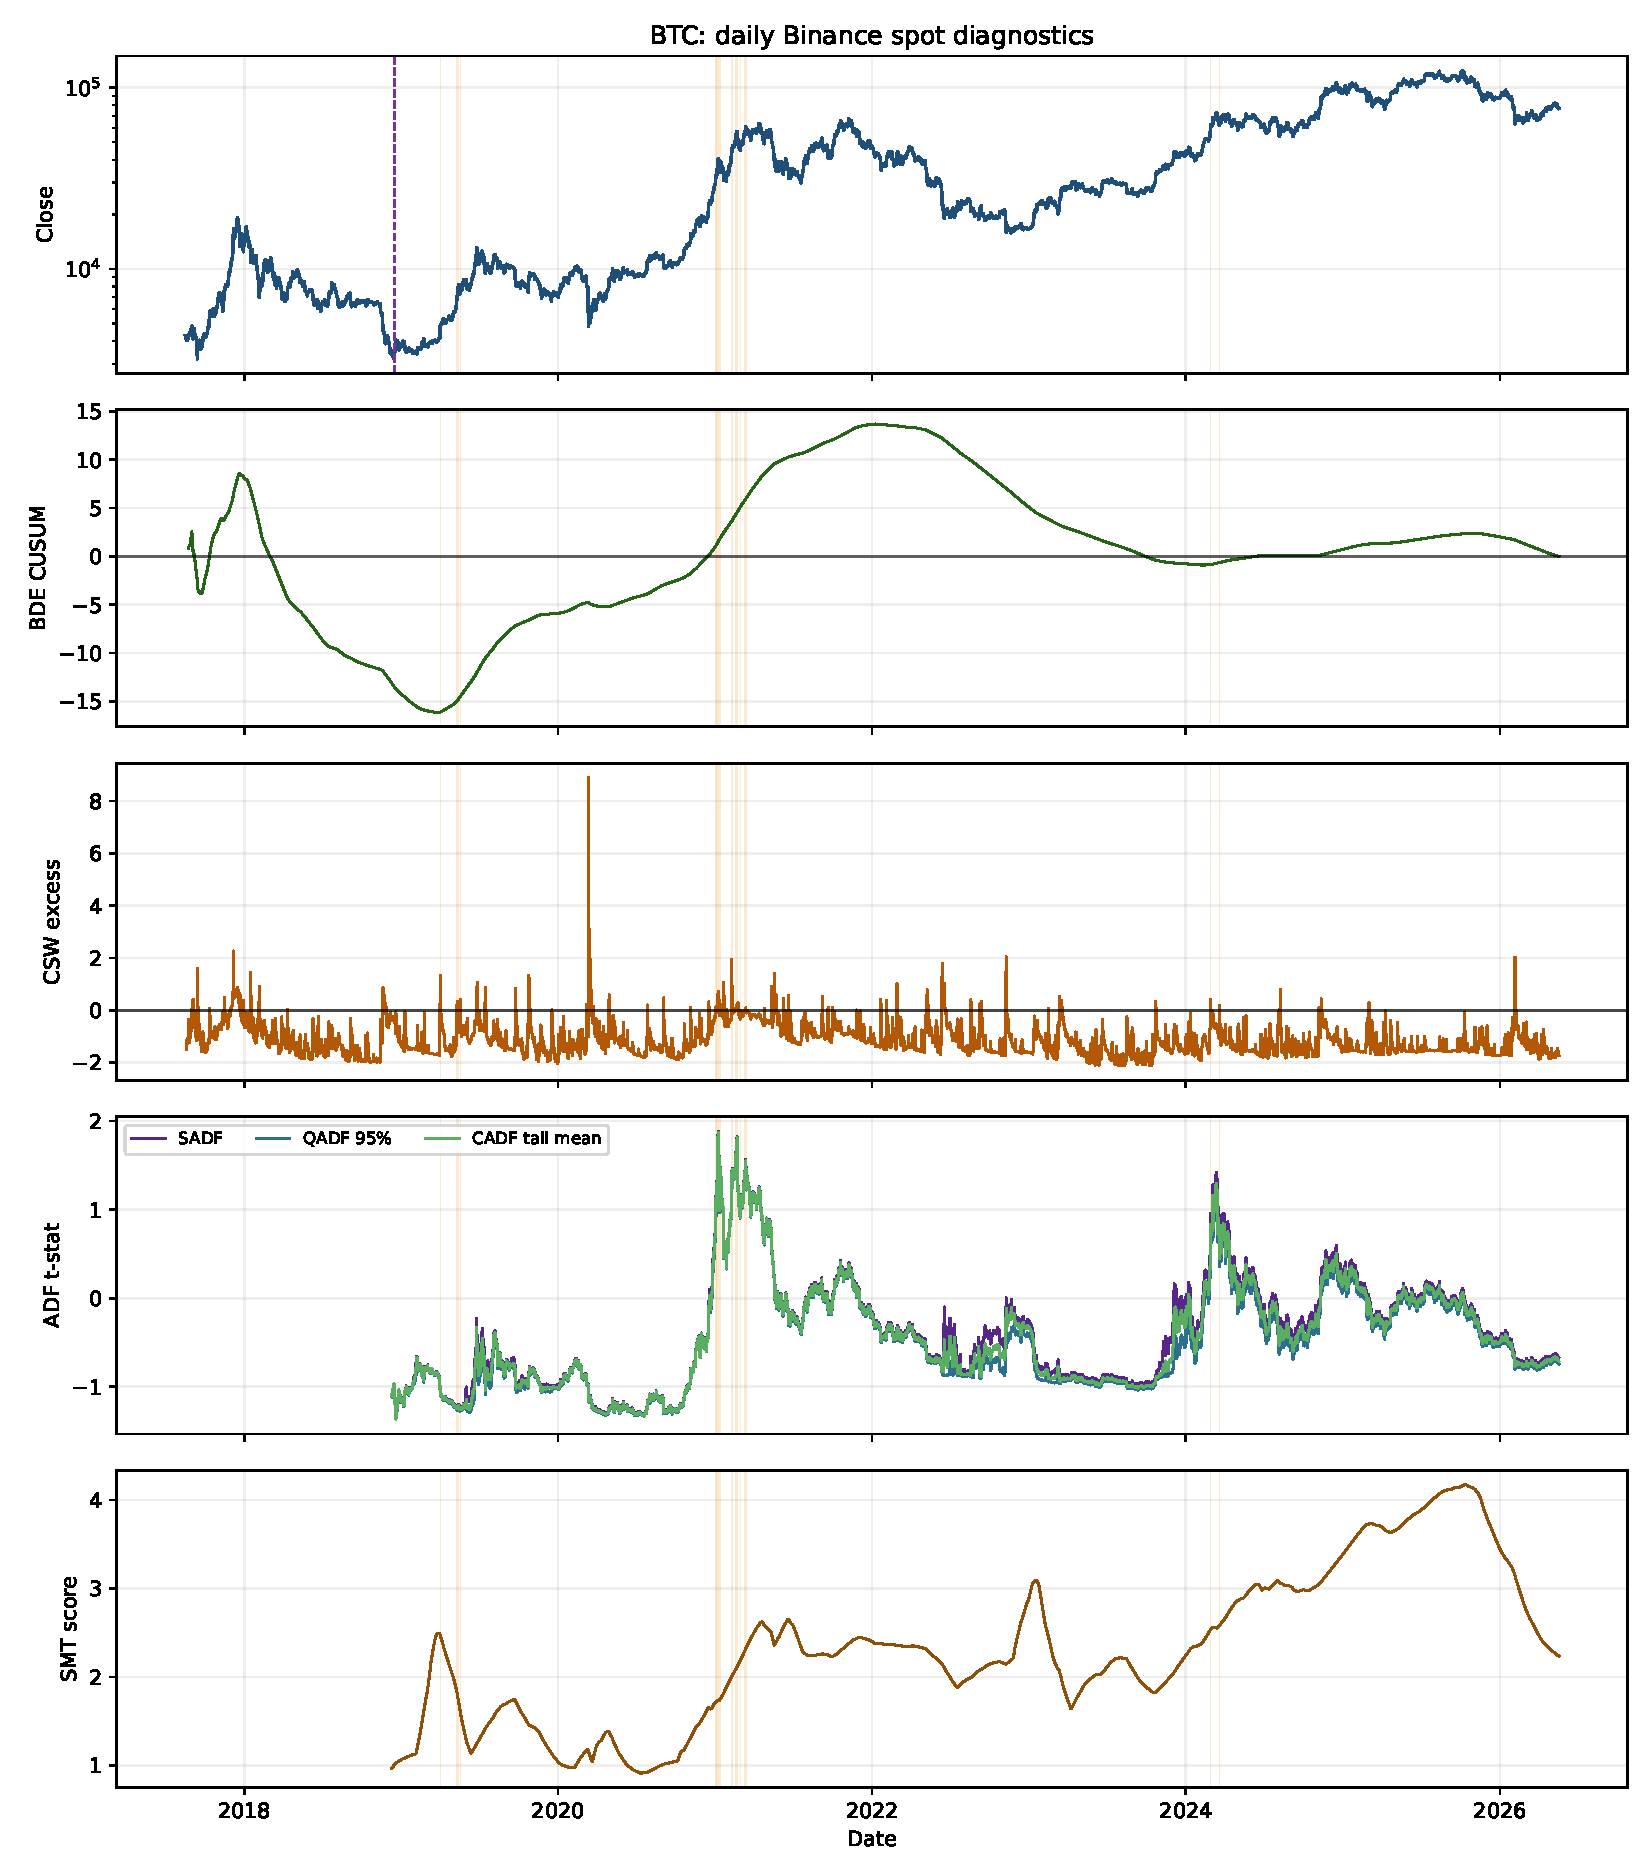
\includegraphics[width=0.98\textwidth]{regime_chapter_figs/fig_asset_BTC.pdf}
\caption{BTC structural-break diagnostics.}
\end{figure}

\subsection{ETH}

24 consensus alert run(s) were detected. The first listed run begins on 2021-01-04. The SDFC candidate date is 2020-03-13, but its t-statistic (0.99) is too small to treat as a formal break call. ETH is the most fragmented long-history asset in this daily run. The largest SADF reading lands in May 2021, while CSW again highlights the March 2020 shock and SMT peaks around the late-2021 trend extension.

\begin{figure}[H]
\centering
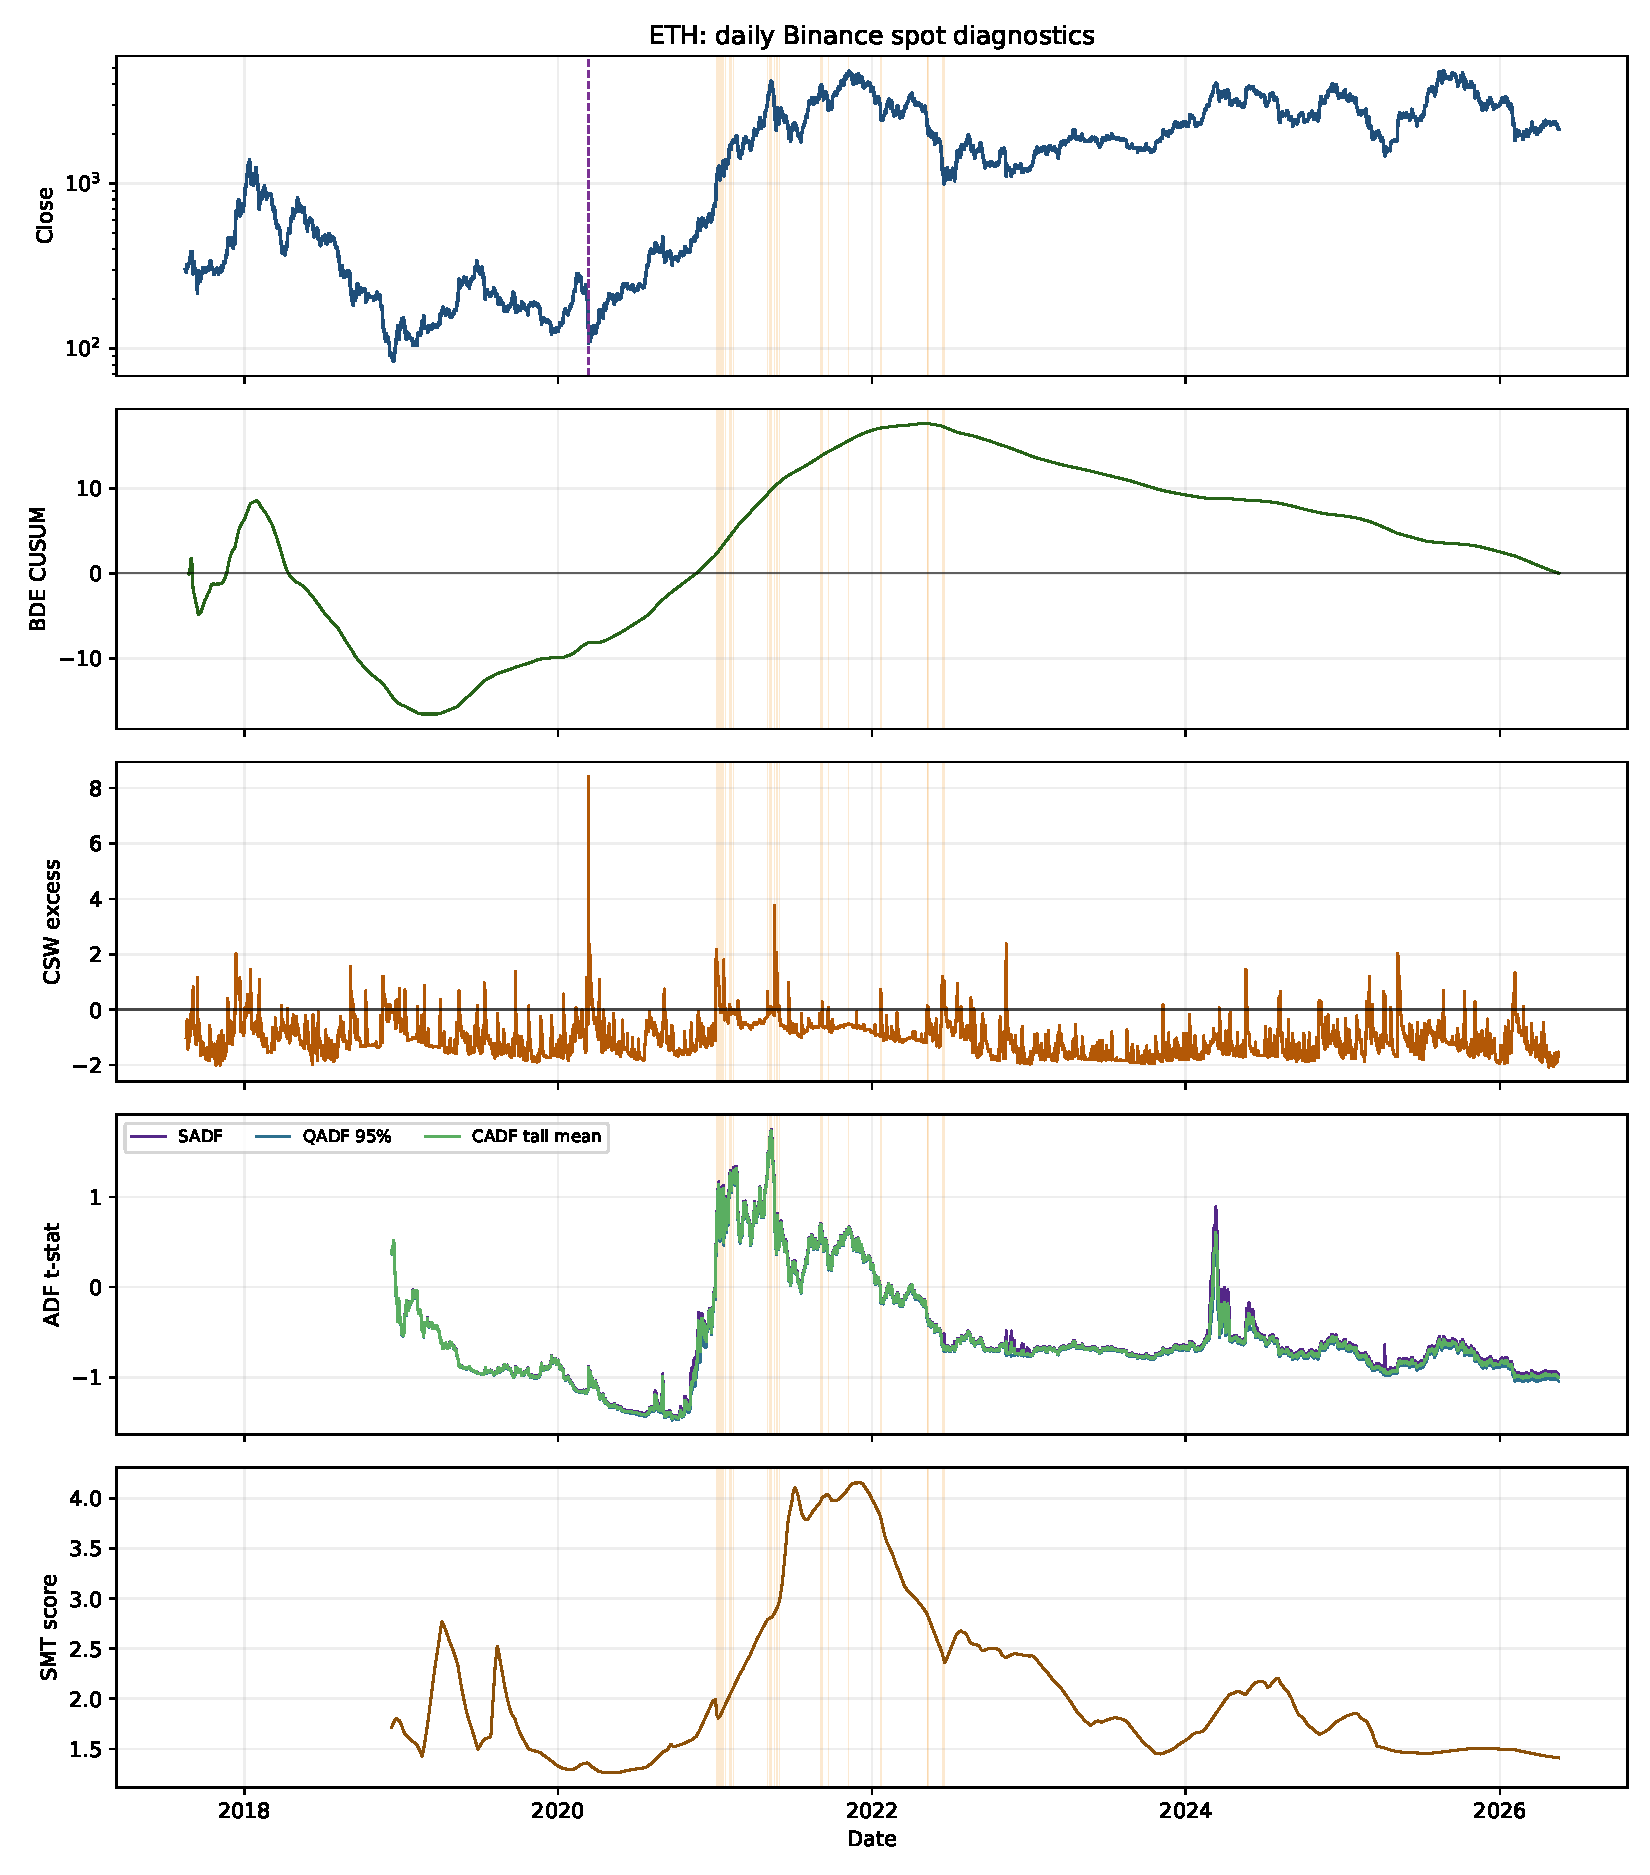
\includegraphics[width=0.98\textwidth]{regime_chapter_figs/fig_asset_ETH.pdf}
\caption{ETH structural-break diagnostics.}
\end{figure}

\subsection{ETC}

8 consensus alert run(s) were detected. The first listed run begins on 2021-04-15. SDFC is not treated as an explosive break for ETC: its best t-statistic is -0.19, which is negative. ETC still concentrates its strongest repeated-window alerts around the 2021 spike and post-spike instability. The daily clock also exposes separate late-2021 and isolated 2022/2024 alert days that are easy to miss at coarser sampling frequencies.

\begin{figure}[H]
\centering
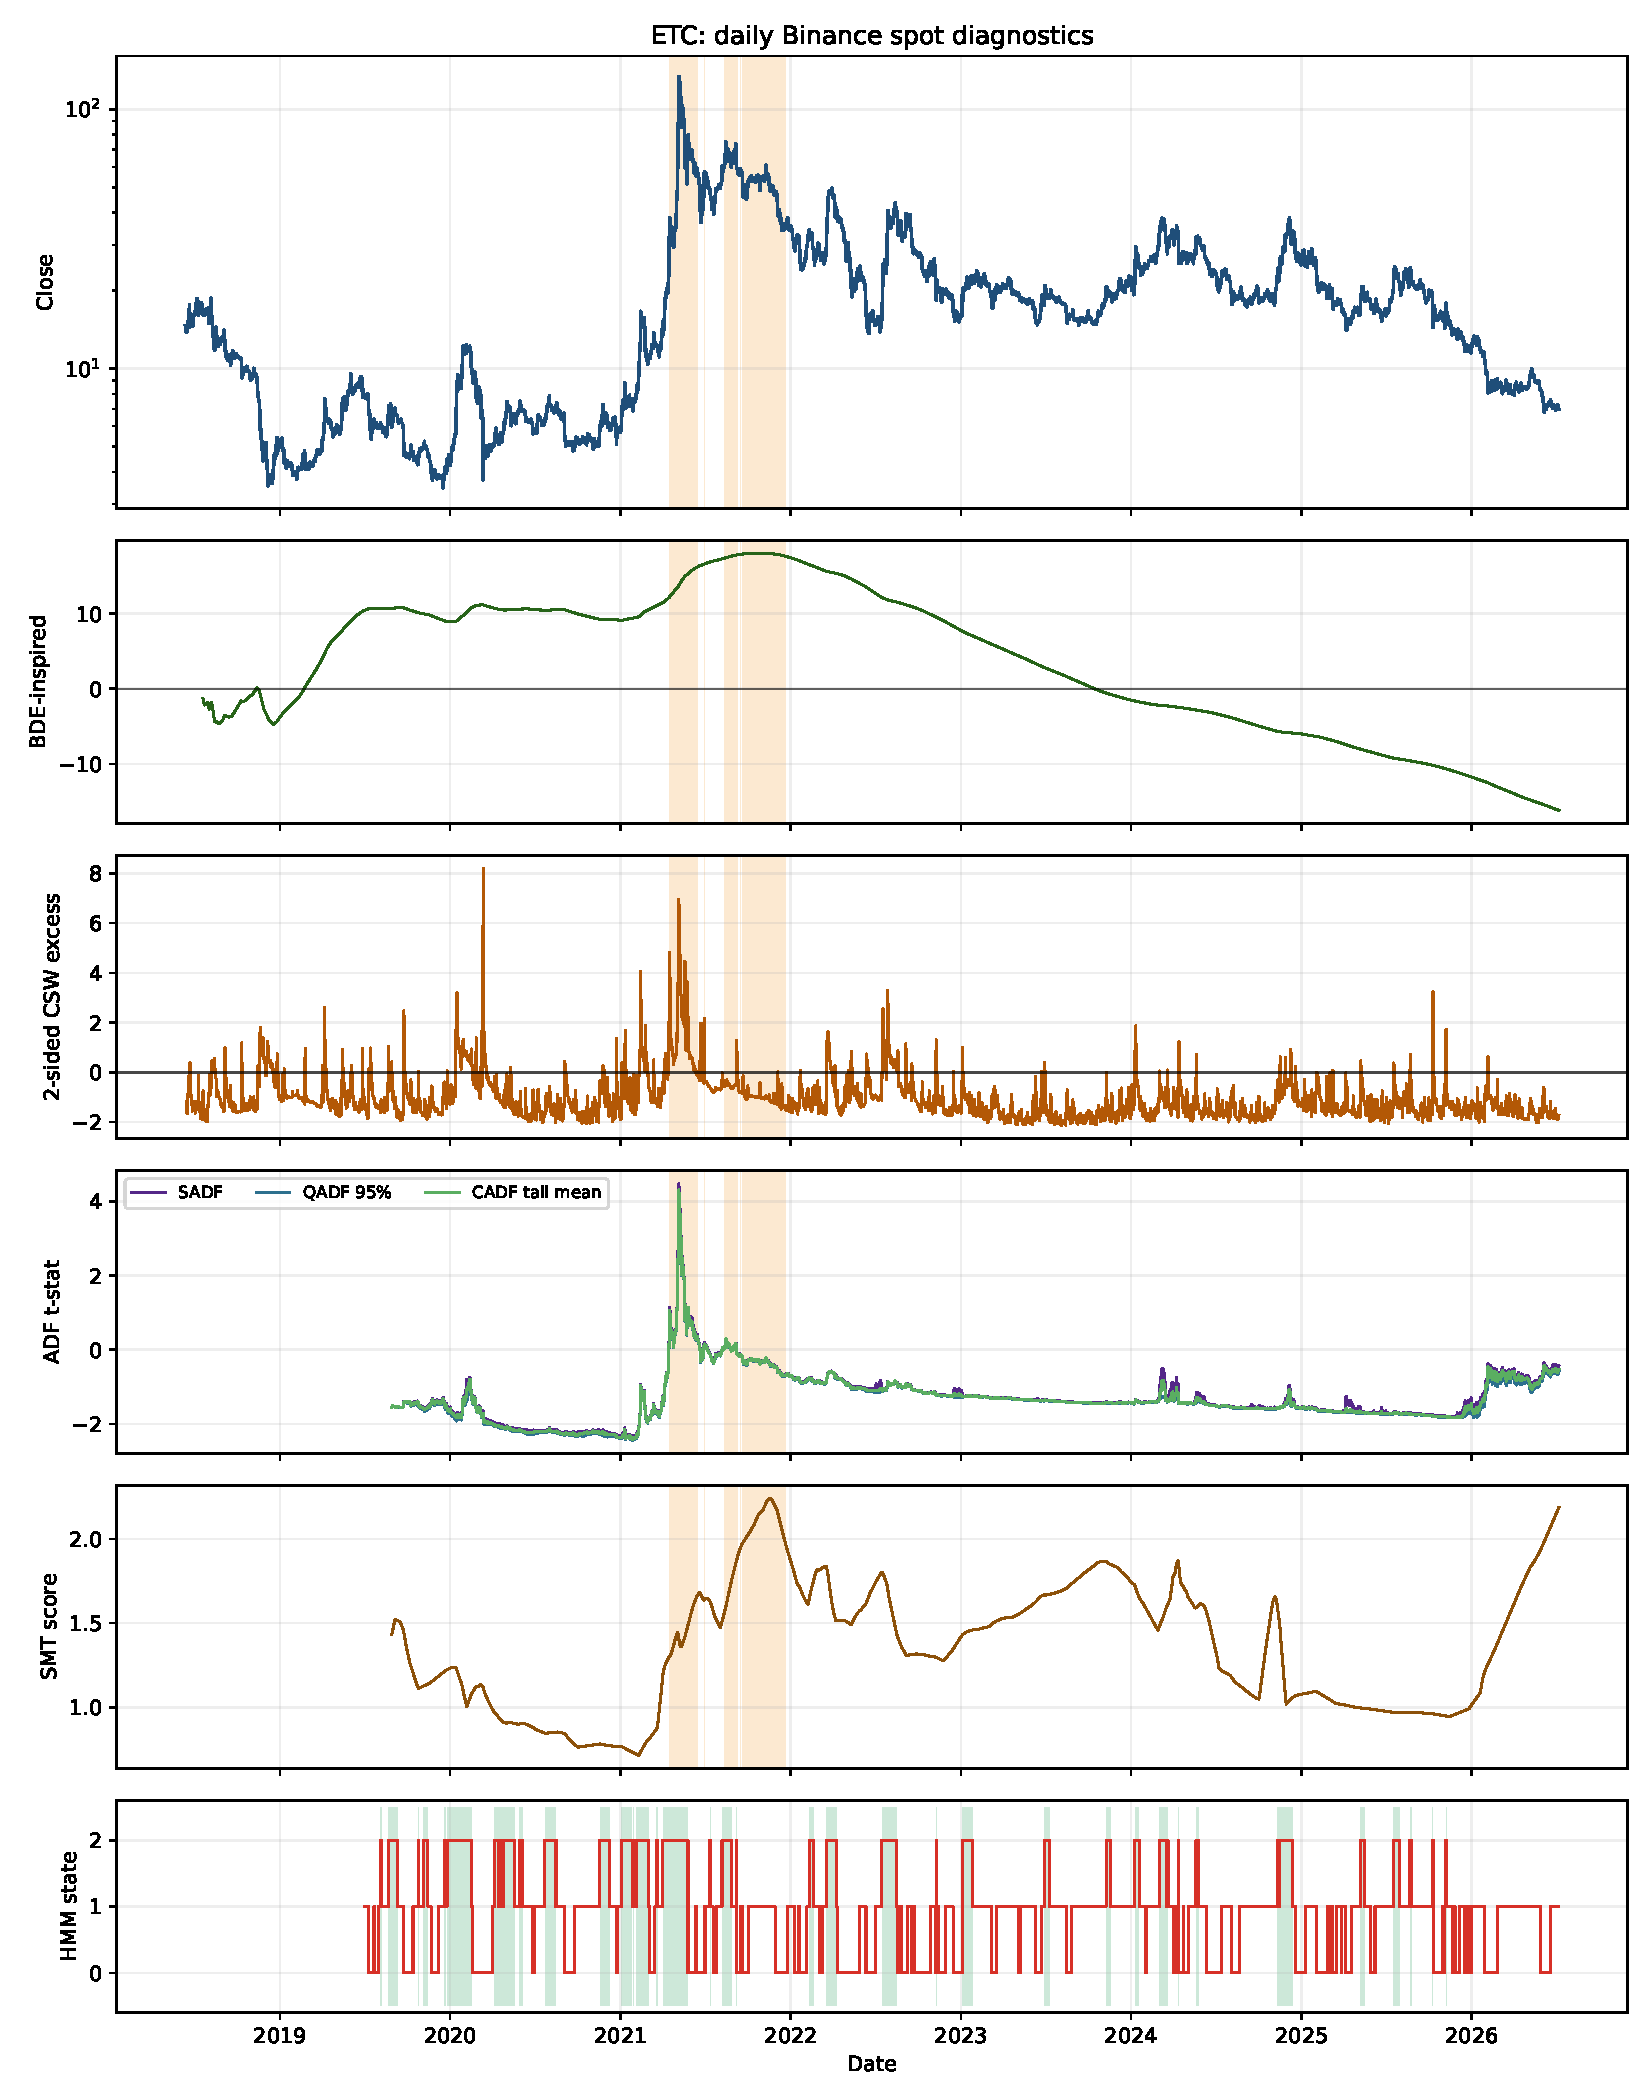
\includegraphics[width=0.98\textwidth]{regime_chapter_figs/fig_asset_ETC.pdf}
\caption{ETC structural-break diagnostics.}
\end{figure}

\subsection{SOL}

9 consensus alert run(s) were detected. The first listed run begins on 2021-04-29. Binance spot SOLUSDT starts on 2020-08-11, so this daily Binance-only sample begins later than the earlier external spreadsheet sample. The SDFC candidate date is 2022-12-30, but its t-statistic (0.62) is too small to treat as a formal break call. SOL's largest SADF reading is in December 2023, while CSW marks the November 2022 collapse and SMT peaks during the January 2023 rebound.

\begin{figure}[H]
\centering
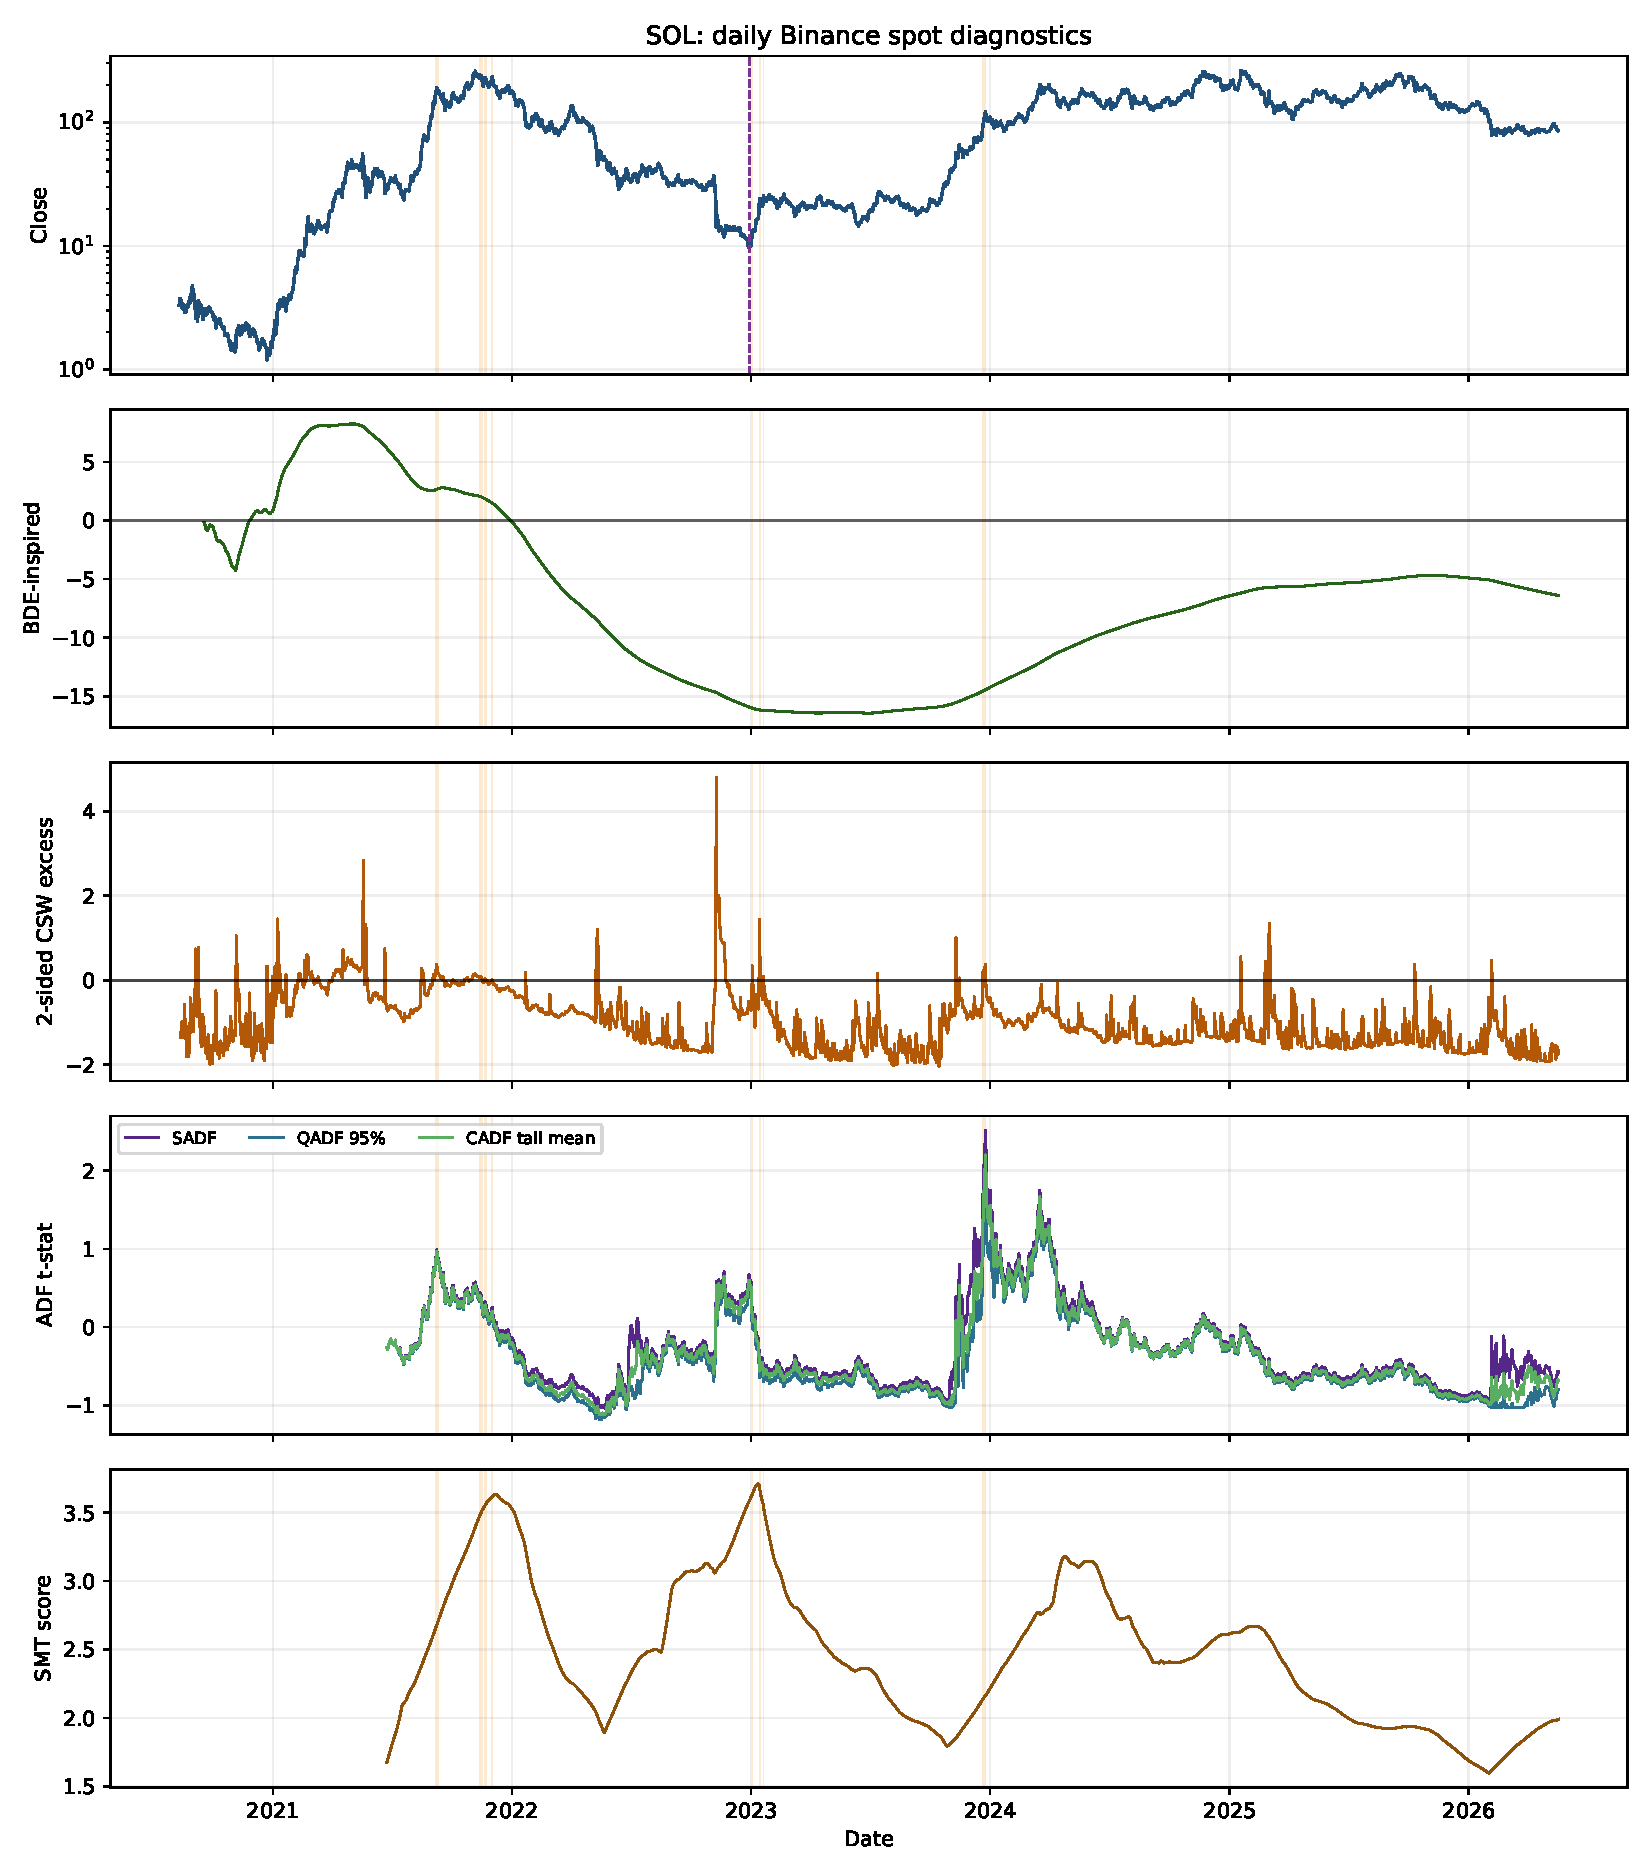
\includegraphics[width=0.98\textwidth]{regime_chapter_figs/fig_asset_SOL.pdf}
\caption{SOL structural-break diagnostics.}
\end{figure}

\subsection{HYPE}

6 consensus alert run(s) were detected. The first listed run begins on 2025-12-18. HYPE is the fallback case: Binance spot HYPEUSDT was unavailable, so the report uses Binance USD-M futures from 2025-05-30 onward. The SDFC candidate date is 2026-01-21, but its t-statistic (1.44) is too small to treat as a formal break call. The history is only 354 daily observations, so its alert clusters should be treated as local research flags rather than stable regime evidence.

\begin{figure}[H]
\centering
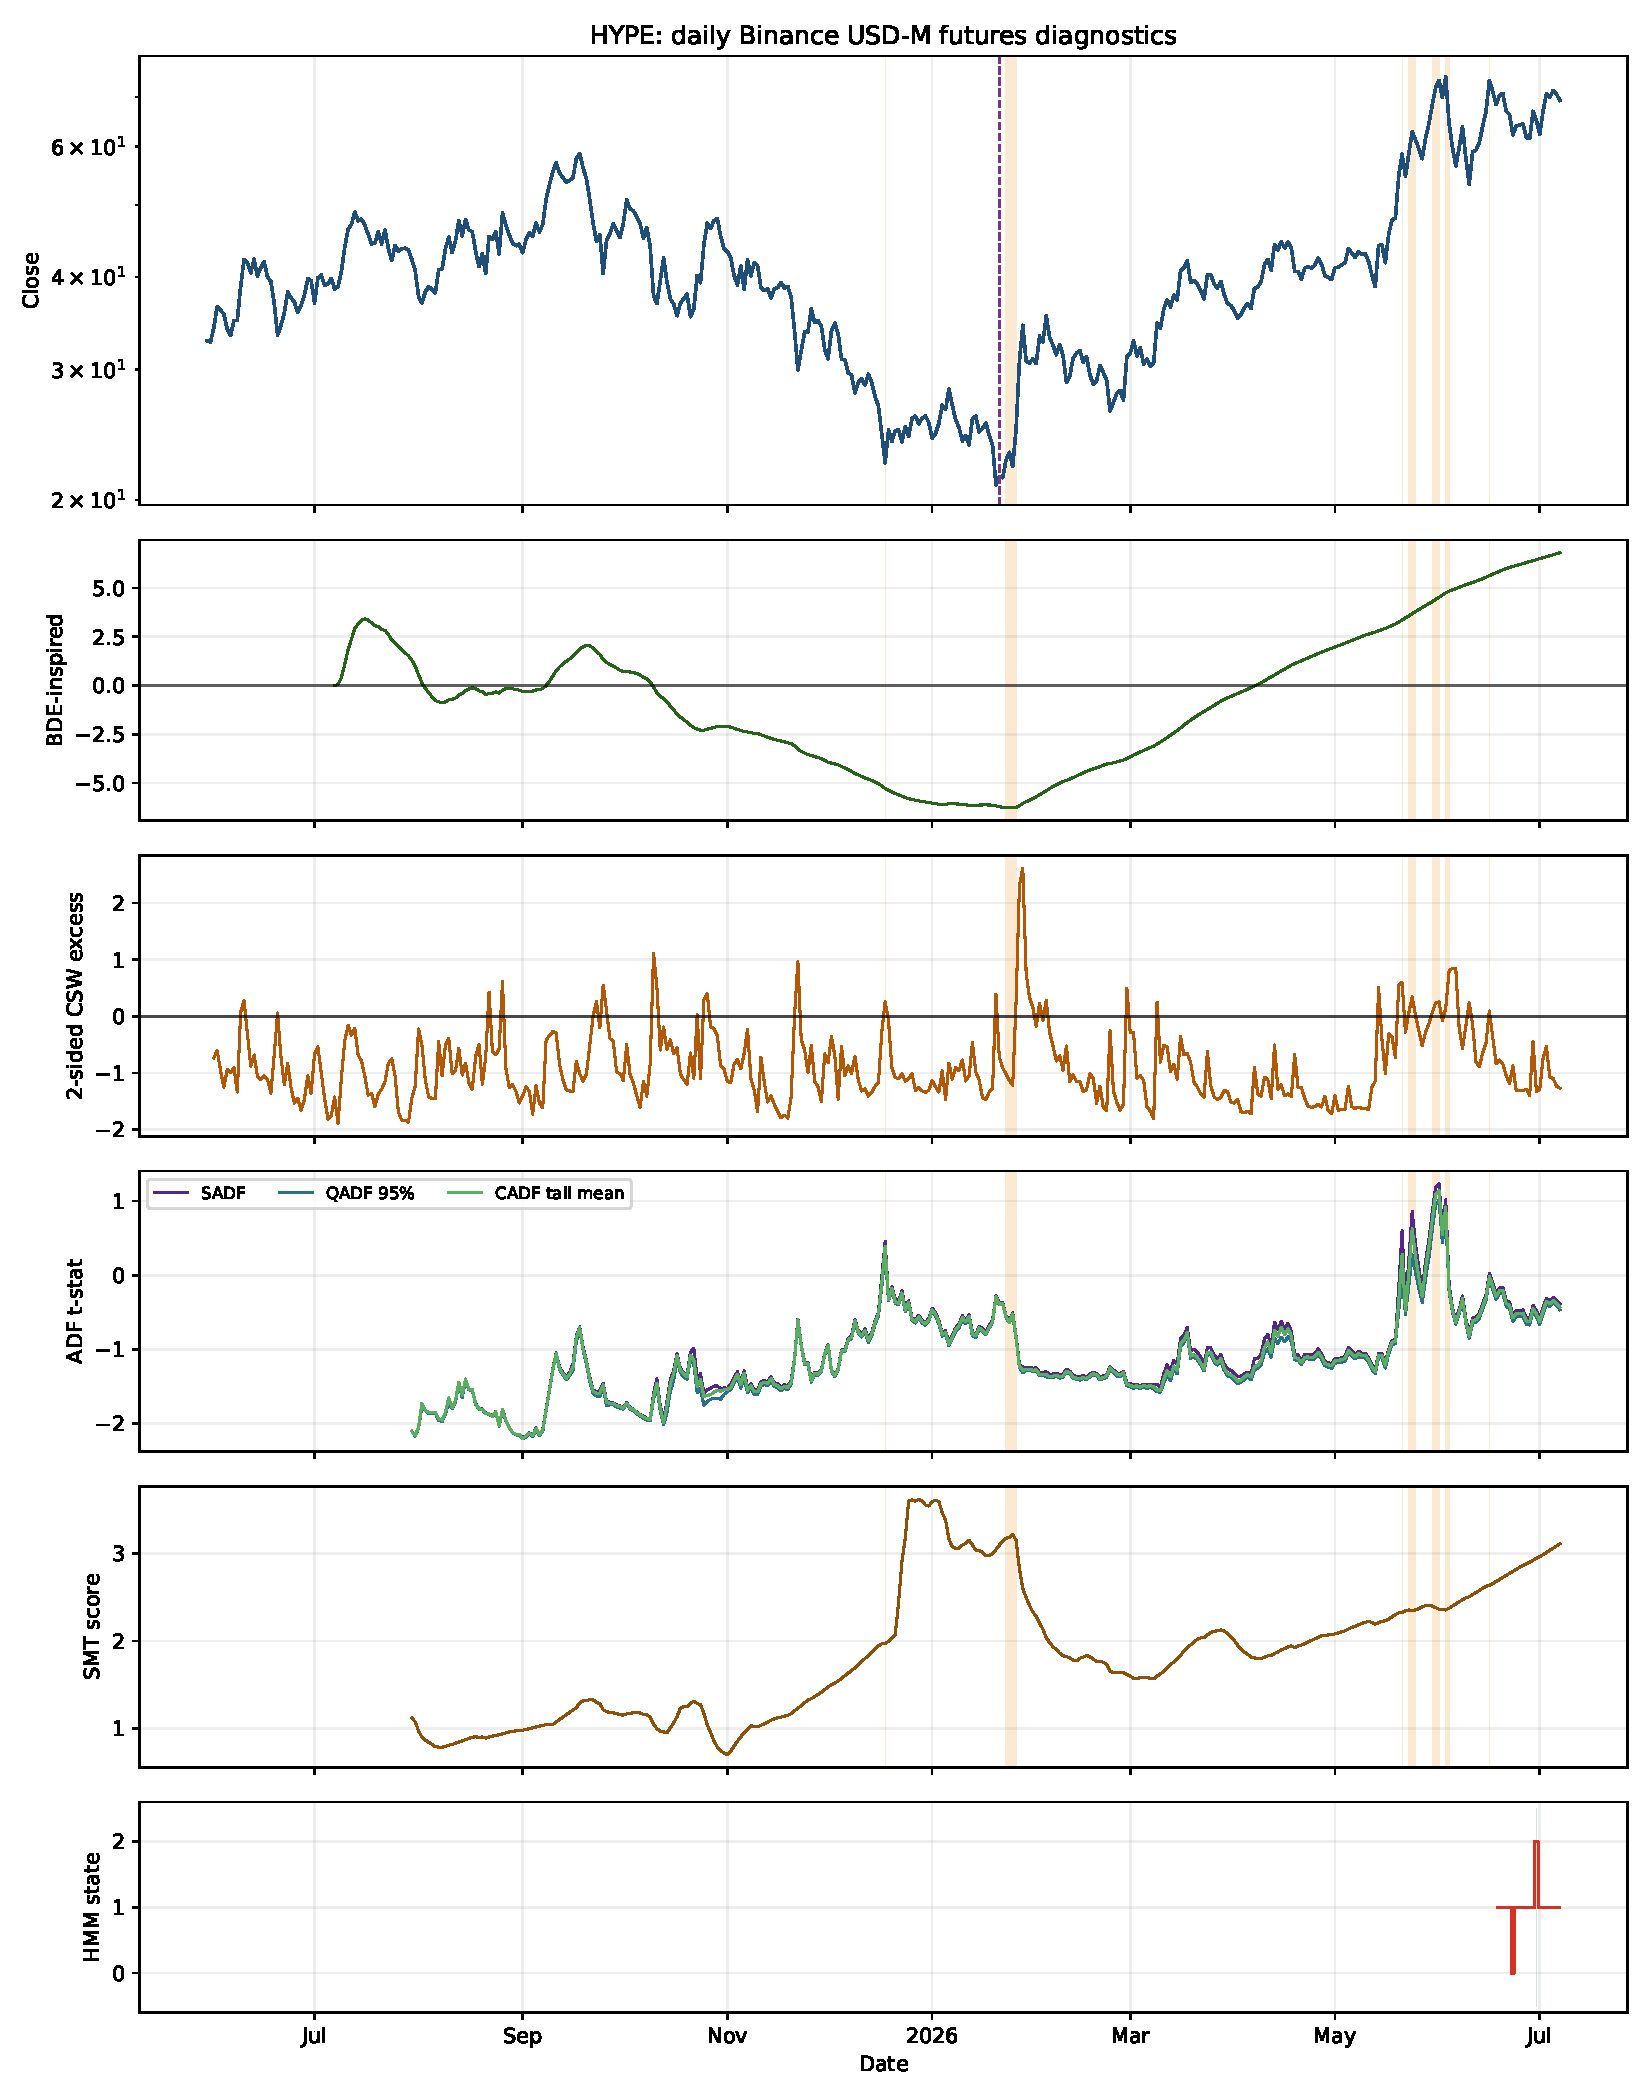
\includegraphics[width=0.98\textwidth]{regime_chapter_figs/fig_asset_HYPE.pdf}
\caption{HYPE structural-break diagnostics.}
\end{figure}

\section{Consensus alert periods}

The table below lists the first few periods in which at least two diagnostic families were active. Short alert runs are common because the tests are sensitive to local trend acceleration and volatility normalization.

\begin{longtable}{@{}lrrr@{}}
\caption{First listed consensus alert periods. Period length is counted in calendar days between the first and last daily alert observation. For assets with many daily runs, the table shows the first eight runs.}\\
\toprule
Asset & Start & End & Days/period length \\
\midrule
\endfirsthead
\toprule
Asset & Start & End & Days/period length \\
\midrule
\endhead
BTC & 2019-04-02 & 2019-04-03 & 2 \\
 & 2019-05-11 & 2019-05-11 & 1 \\
 & 2019-05-13 & 2019-05-15 & 3 \\
 & 2019-05-19 & 2019-05-19 & 1 \\
 & 2021-01-02 & 2021-01-03 & 2 \\
 & 2021-01-05 & 2021-01-10 & 6 \\
 & 2021-01-13 & 2021-01-14 & 2 \\
 & 2021-02-08 & 2021-02-09 & 2 \\
ETH & 2021-01-04 & 2021-01-10 & 7 \\
 & 2021-01-14 & 2021-01-14 & 1 \\
 & 2021-01-16 & 2021-01-16 & 1 \\
 & 2021-01-19 & 2021-01-20 & 2 \\
 & 2021-01-24 & 2021-01-24 & 1 \\
 & 2021-02-03 & 2021-02-03 & 1 \\
 & 2021-02-05 & 2021-02-05 & 1 \\
 & 2021-02-08 & 2021-02-09 & 2 \\
ETC & 2021-04-15 & 2021-06-11 & 58 \\
 & 2021-06-13 & 2021-06-14 & 2 \\
 & 2021-06-29 & 2021-06-30 & 2 \\
 & 2021-09-02 & 2021-09-09 & 8 \\
 & 2021-10-28 & 2021-12-23 & 57 \\
 & 2022-01-22 & 2022-01-22 & 1 \\
 & 2022-04-06 & 2022-04-06 & 1 \\
 & 2024-04-12 & 2024-04-12 & 1 \\
SOL & 2021-04-29 & 2021-05-20 & 22 \\
 & 2021-05-22 & 2021-05-24 & 3 \\
 & 2021-06-21 & 2021-06-21 & 1 \\
 & 2021-09-07 & 2021-09-11 & 5 \\
 & 2021-10-31 & 2021-12-02 & 33 \\
 & 2023-01-03 & 2023-01-03 & 1 \\
 & 2023-01-14 & 2023-01-16 & 3 \\
 & 2023-01-20 & 2023-01-20 & 1 \\
HYPE & 2025-12-18 & 2025-12-18 & 1 \\
 & 2025-12-23 & 2025-12-25 & 3 \\
 & 2026-01-01 & 2026-01-02 & 2 \\
 & 2026-01-20 & 2026-01-22 & 3 \\
 & 2026-01-26 & 2026-01-31 & 6 \\
 & 2026-02-02 & 2026-02-02 & 1 \\
\bottomrule
\end{longtable}

\begin{figure}[H]
\centering
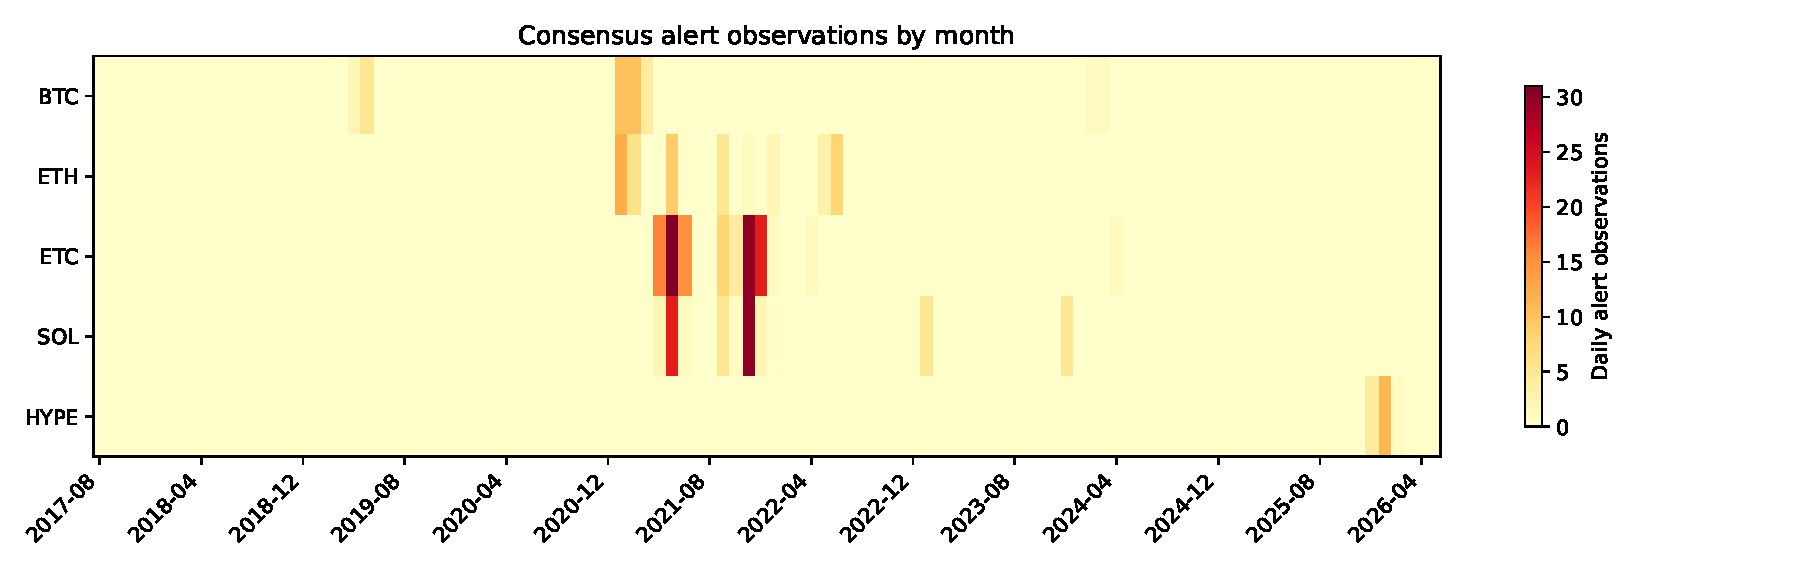
\includegraphics[width=0.98\textwidth]{regime_chapter_figs/fig02_alert_heatmap.pdf}
\caption{Consensus-alert density by calendar month. A darker cell means more alert observations occurred in that month for that asset.}
\end{figure}

\section{Simple long/flat trading evaluation}

The diagnostics above are research features, not trading rules. Still, it is useful to ask the practical question: \emph{if a structural-break indicator is meant to identify tradable regime changes, what would a very simple long-or-cash rule have done?}

\subsection{Backtest rule}

The strategy conversion is deliberately simple and cautious:
\begin{enumerate}
    \item At each daily close $t$, compute the diagnostics using data through $t$ only.
    \item Convert each indicator into an online alert. BDE, SADF, QADF, CADF, and SMT alert when the current value is above its prior expanding 95th percentile, after at least 60 prior finite observations. CSW alerts when its excess is positive, because it already embeds the Chapter 17 critical curve.
    \item Require the trailing 20-day log return to be positive. This momentum gate avoids going long on structural-break alerts that are mostly crash or liquidation warnings.
    \item Enter long on the next daily close-to-close return, not the same day's return. This one-day shift avoids same-close look-ahead.
    \item Keep the position long for 20 trading days after a valid alert, then move back out of the market unless a new alert refreshes the holding window.
    \item Charge 10 basis points whenever exposure changes. The buy-and-hold baseline is shown without turnover costs.
\end{enumerate}

SDFC is not traded in this exercise because it is a full-sample unknown-break diagnostic. Trading it directly would use future data to choose the break date. The ``Consensus'' strategy is long when at least two of BDE, CSW, SADF, and SMT fire on the same close, subject to the same momentum gate and 20-day holding window.

This is still an in-sample comparison. The best final PnL is therefore only an indicative ranking of which simple signal conversion looked promising on this sample, not evidence of a deployable strategy.

\begin{table}[H]
\centering
\scriptsize
\setlength{\tabcolsep}{4pt}
\resizebox{\textwidth}{!}{%
\begin{tabular}{@{}llrrlrrr@{}}
\toprule
Asset & Best structure signal & Best signal final & Buy-and-hold final & Best including buy-and-hold & Max DD & Exposure & Trades \\
\midrule
BTC & CSW & 11.68x & 17.97x & Buy-and-hold & -37\% & 17\% & 20 \\
ETH & CADF & 3.78x & 7.05x & Buy-and-hold & -50\% & 5\% & 1 \\
ETC & CSW & 11.44x & 0.61x & CSW & -67\% & 26\% & 24 \\
SOL & Consensus & 35.57x & 25.88x & Consensus & -56\% & 16\% & 5 \\
HYPE & CSW & 1.09x & 1.45x & Buy-and-hold & -46\% & 38\% & 7 \\
\bottomrule
\end{tabular}}
\caption{Best long/flat structure-break strategy by final equity multiple. ``Best structure signal'' excludes buy-and-hold; ``Best including buy-and-hold'' includes it. Max DD, exposure, and trades refer to the best structure signal.}
\end{table}

\begin{figure}[H]
\centering
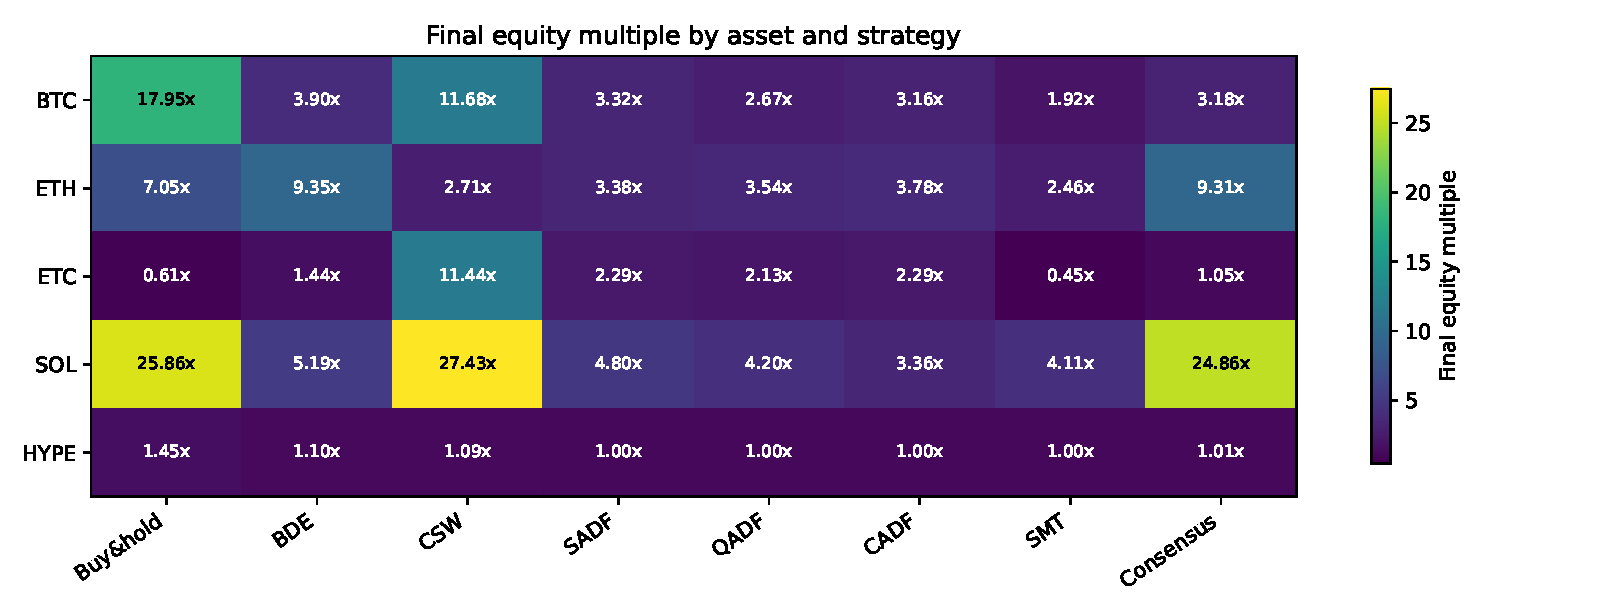
\includegraphics[width=0.98\textwidth]{regime_chapter_figs/fig_strategy_final_multiple_heatmap.pdf}
\caption{Final equity multiple by asset and strategy. Values are in-sample and normalized to 1 at each asset's first available observation.}
\end{figure}

\subsection{PnL curves by asset}

\begin{figure}[H]
\centering
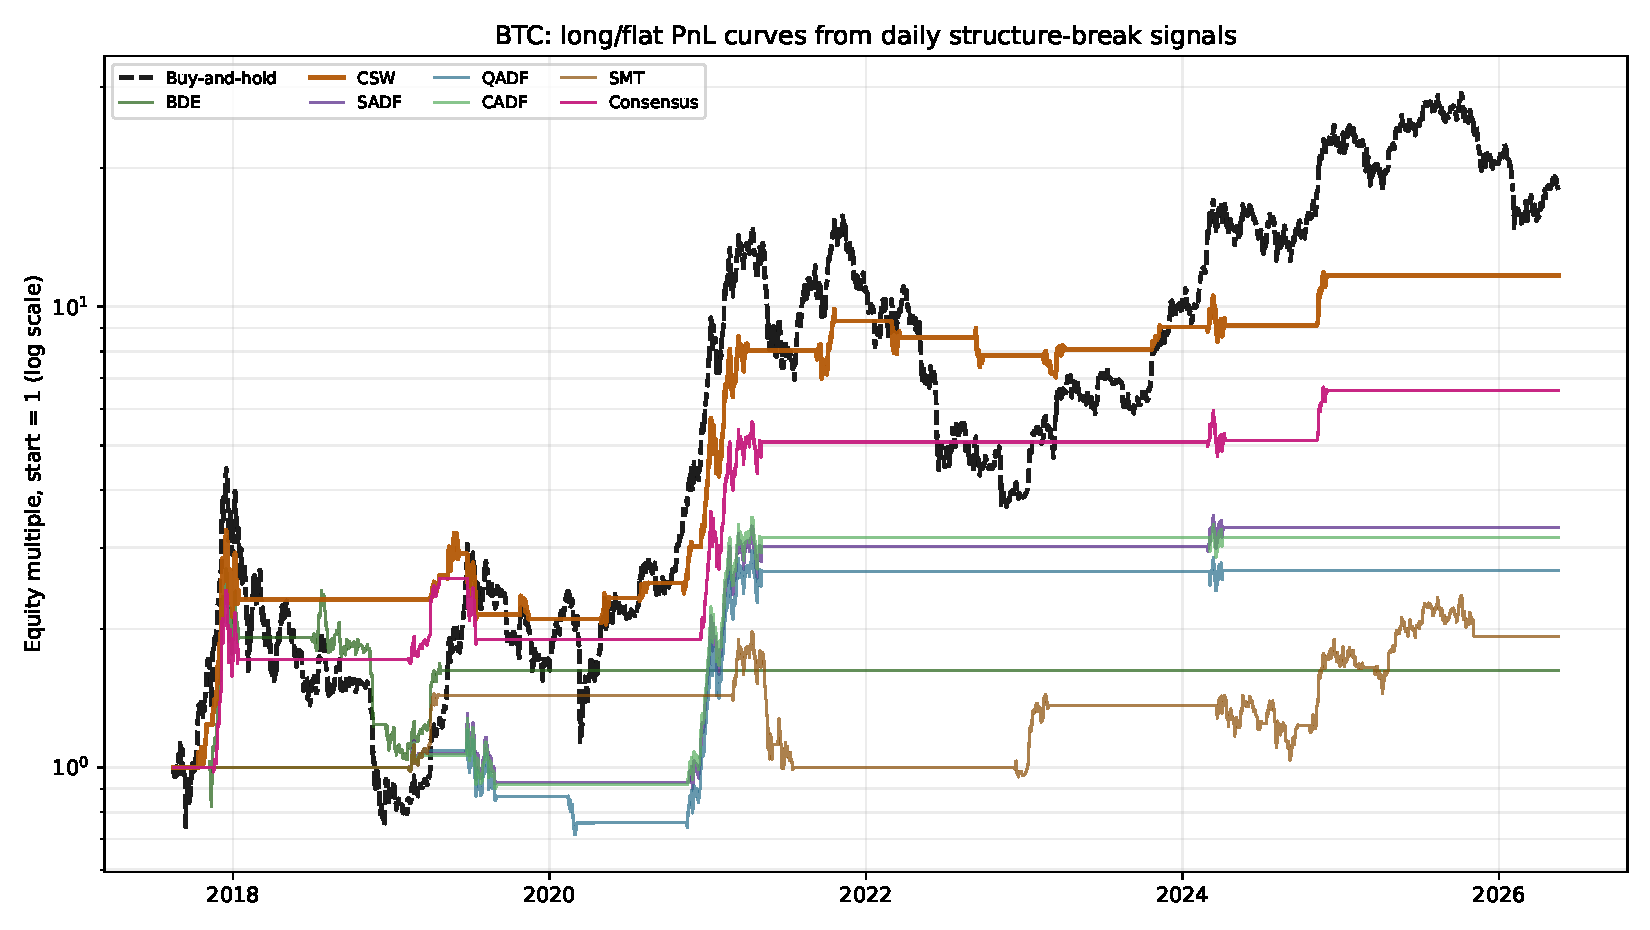
\includegraphics[width=0.98\textwidth]{regime_chapter_figs/fig_strategy_pnl_BTC.pdf}
\caption{BTC long/flat strategy PnL curves.}
\end{figure}

\begin{figure}[H]
\centering
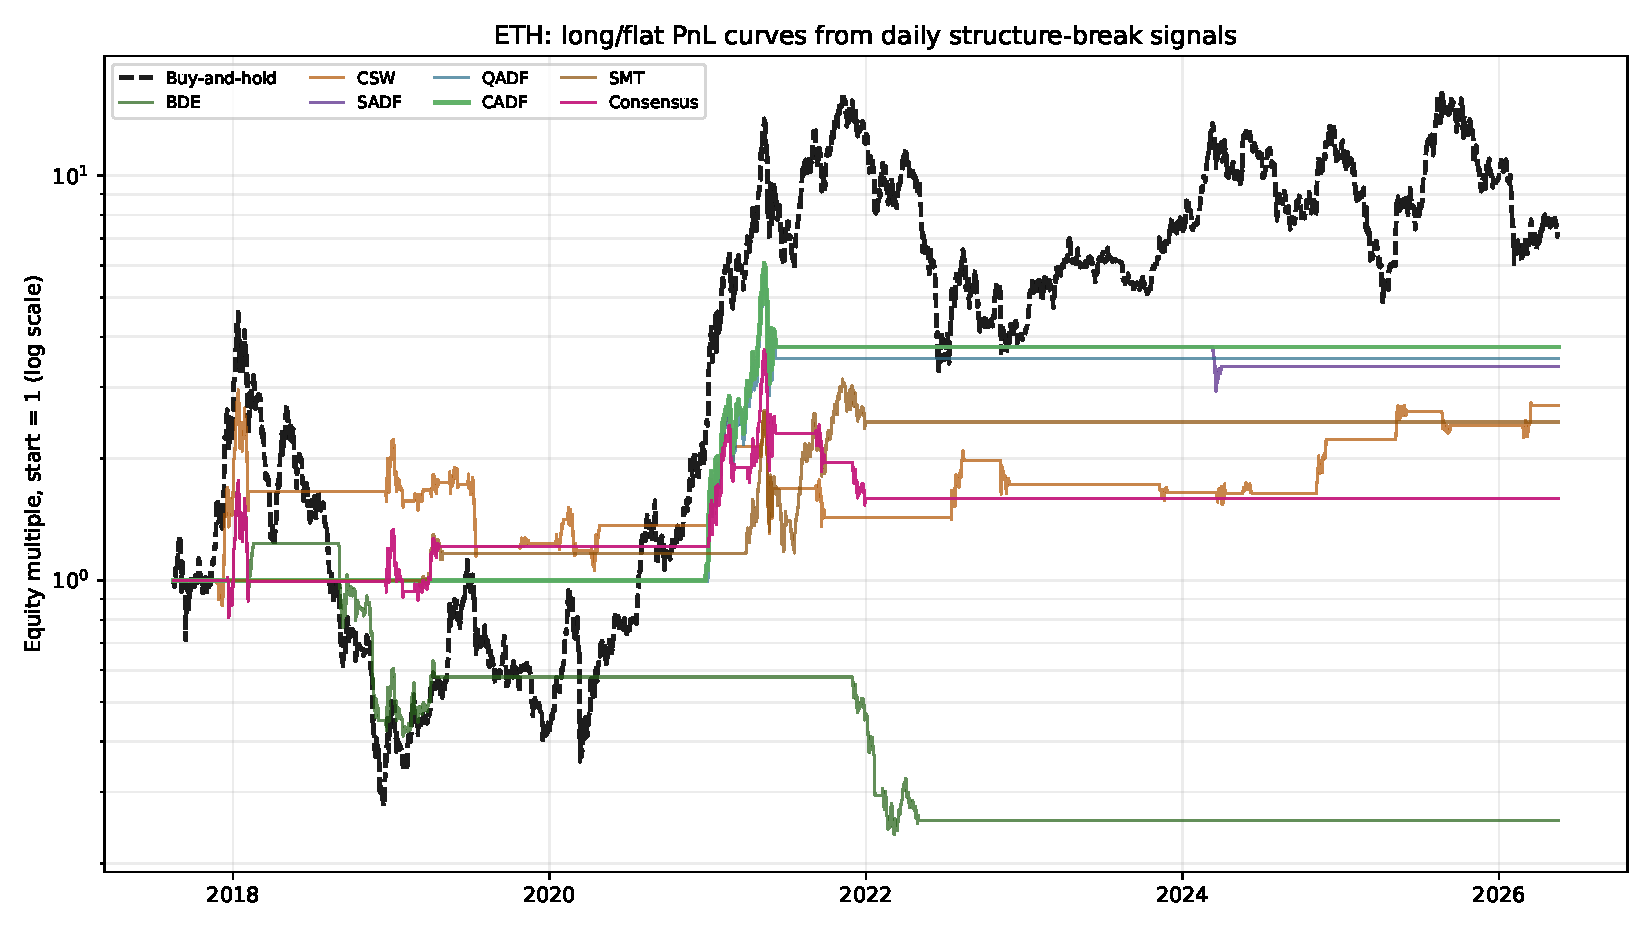
\includegraphics[width=0.98\textwidth]{regime_chapter_figs/fig_strategy_pnl_ETH.pdf}
\caption{ETH long/flat strategy PnL curves.}
\end{figure}

\begin{figure}[H]
\centering
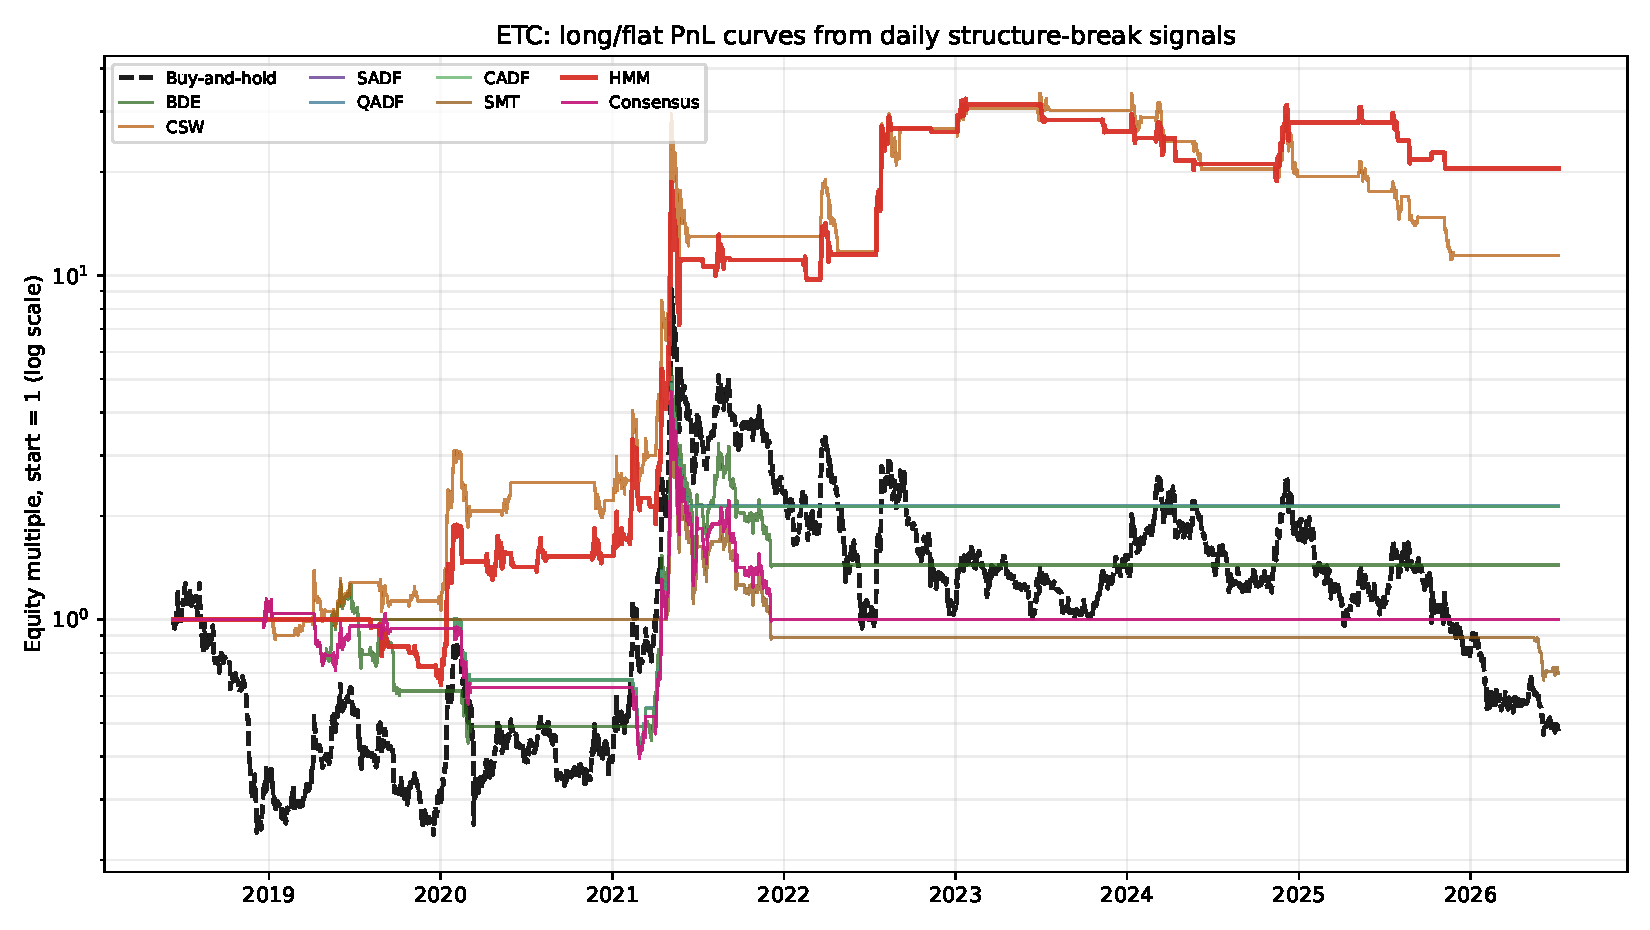
\includegraphics[width=0.98\textwidth]{regime_chapter_figs/fig_strategy_pnl_ETC.pdf}
\caption{ETC long/flat strategy PnL curves.}
\end{figure}

\begin{figure}[H]
\centering
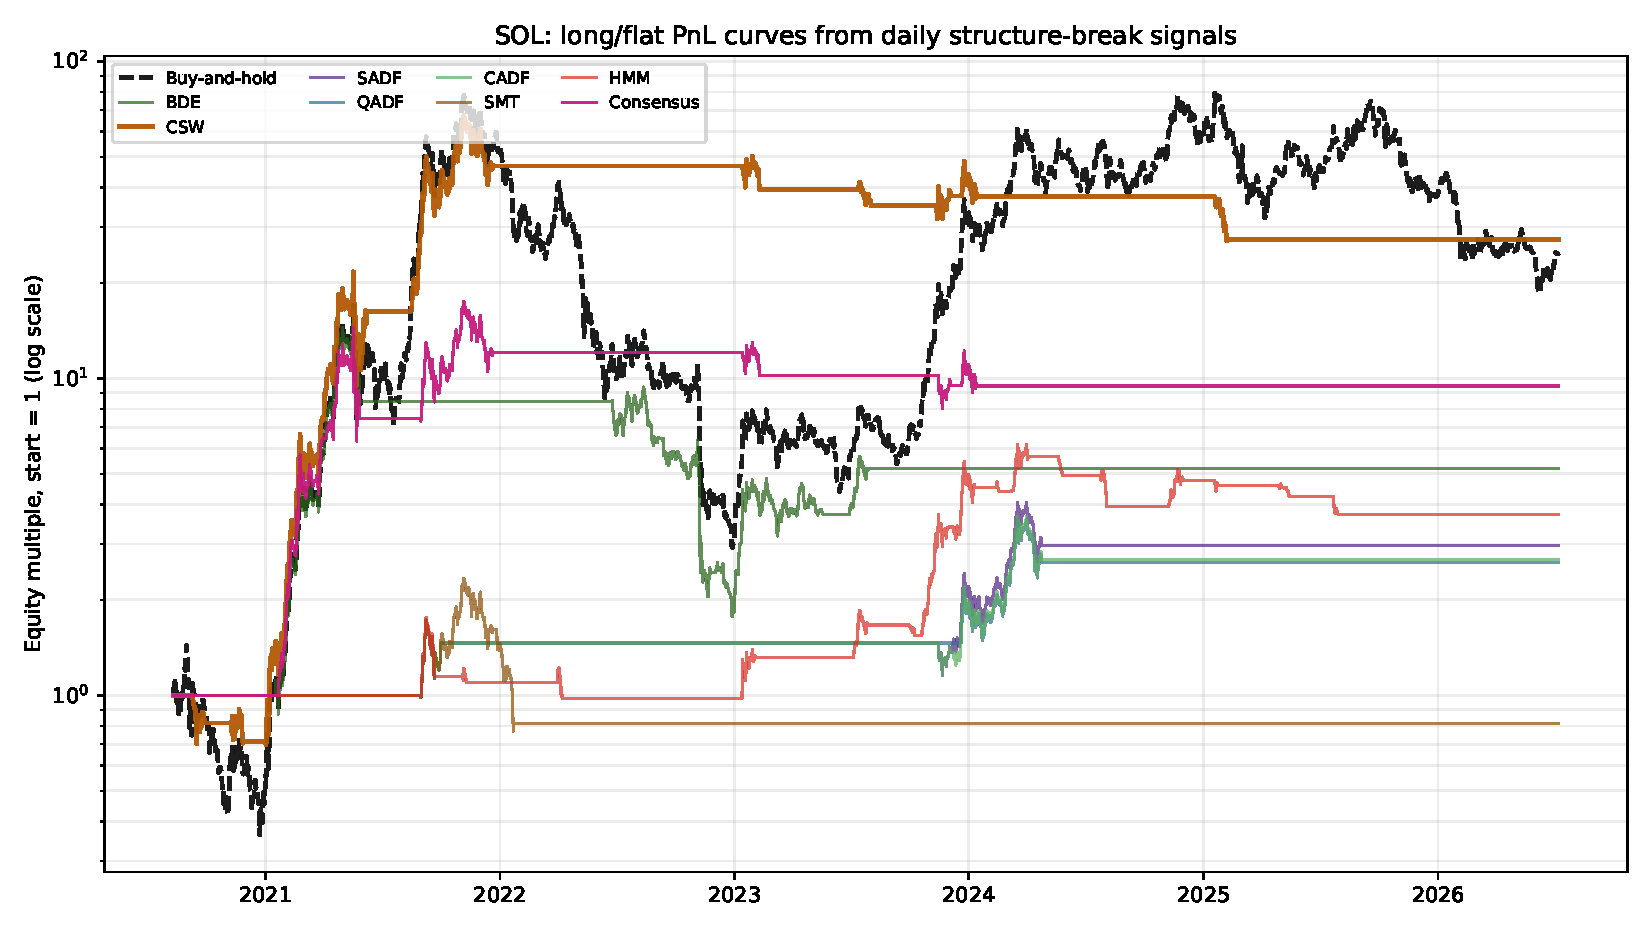
\includegraphics[width=0.98\textwidth]{regime_chapter_figs/fig_strategy_pnl_SOL.pdf}
\caption{SOL long/flat strategy PnL curves.}
\end{figure}

\begin{figure}[H]
\centering
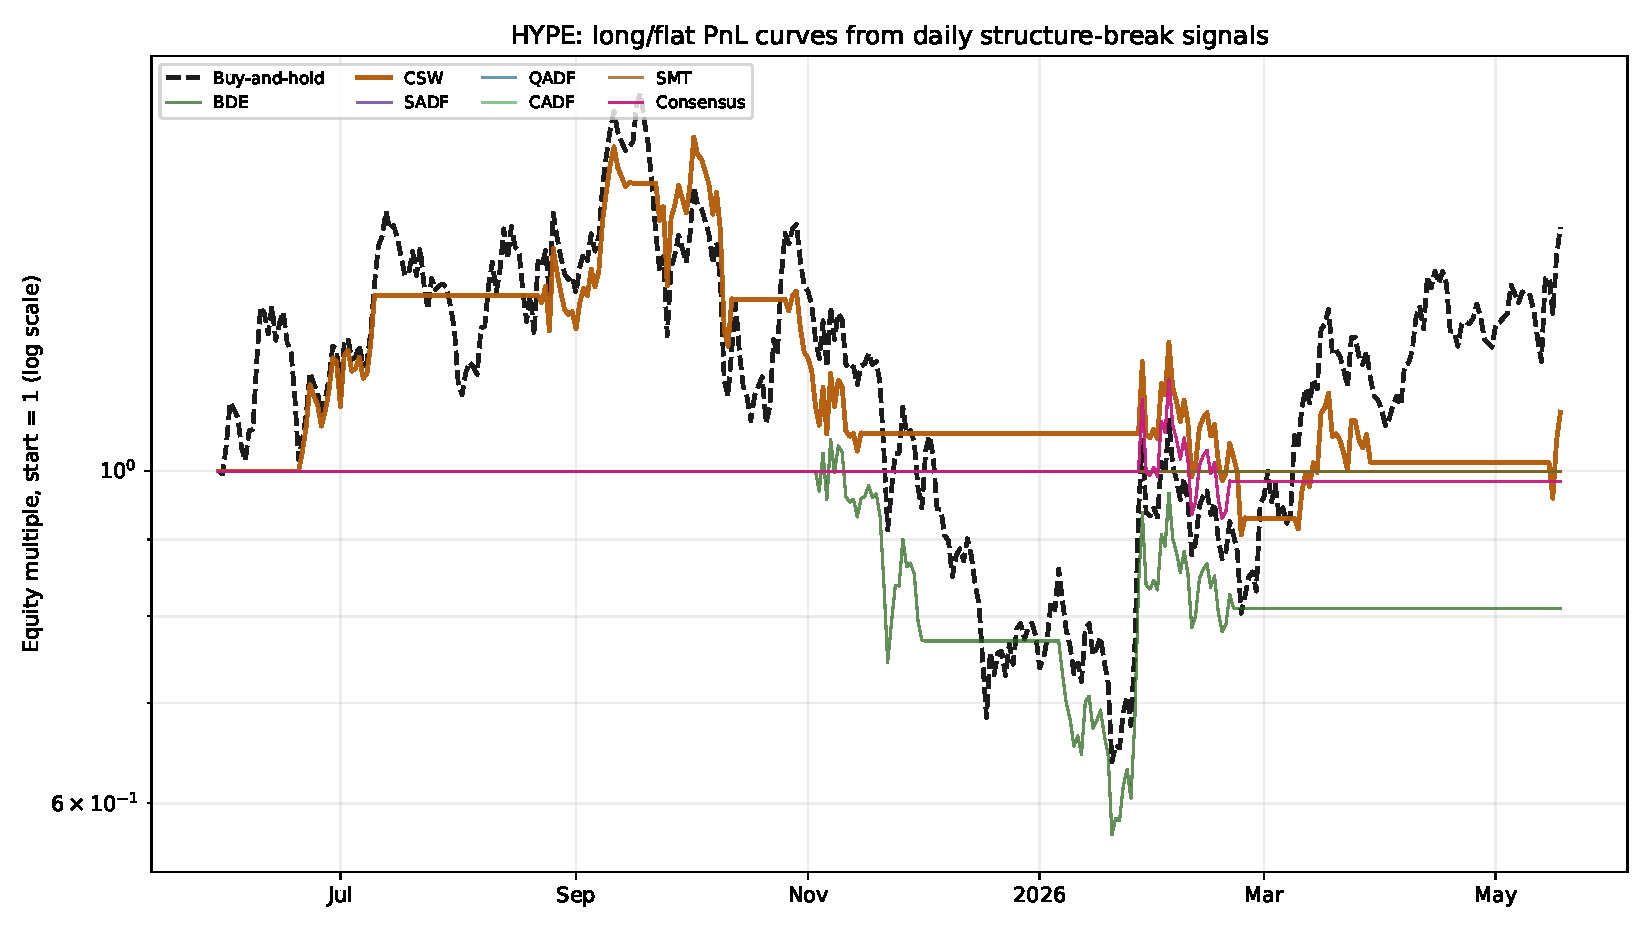
\includegraphics[width=0.98\textwidth]{regime_chapter_figs/fig_strategy_pnl_HYPE.pdf}
\caption{HYPE long/flat strategy PnL curves, using Binance USD-M futures because Binance spot HYPEUSDT was unavailable.}
\end{figure}

\subsection{Full strategy table}

\begin{longtable}{@{}llrrrrrrr@{}}
\caption{Simple long/flat strategy performance. Final multiple is the ending equity multiple from 1. CAGR is annualized over each asset's available sample, so HYPE's short history makes its annualized values especially unstable. Sharpe uses daily returns and 365-day annualization.}\\
\toprule
Asset & Strategy & Final & Total return & CAGR & Max DD & Sharpe & Exposure & Trades \\
\midrule
\endfirsthead
\toprule
Asset & Strategy & Final & Total return & CAGR & Max DD & Sharpe & Exposure & Trades \\
\midrule
\endhead
BTC & Buy-and-hold & 17.97x & 1697\% & 39\% & -83\% & 0.83 & 100\% & 1 \\
BTC & BDE & 1.63x & 63\% & 6\% & -61\% & 0.34 & 11\% & 4 \\
BTC & CSW & 11.68x & 1068\% & 32\% & -37\% & 1.00 & 17\% & 20 \\
BTC & SADF & 3.32x & 232\% & 15\% & -31\% & 0.66 & 9\% & 5 \\
BTC & QADF & 2.67x & 167\% & 12\% & -41\% & 0.56 & 11\% & 6 \\
BTC & CADF & 3.16x & 216\% & 14\% & -30\% & 0.64 & 9\% & 5 \\
BTC & SMT & 1.92x & 92\% & 8\% & -52\% & 0.41 & 25\% & 11 \\
BTC & Consensus & 6.58x & 558\% & 24\% & -35\% & 0.86 & 11\% & 7 \\
ETH & Buy-and-hold & 7.05x & 605\% & 25\% & -94\% & 0.70 & 100\% & 1 \\
ETH & BDE & 0.26x & -74\% & -14\% & -87\% & -0.26 & 12\% & 9 \\
ETH & CSW & 2.71x & 171\% & 12\% & -64\% & 0.48 & 18\% & 22 \\
ETH & SADF & 3.38x & 238\% & 15\% & -52\% & 0.61 & 6\% & 2 \\
ETH & QADF & 3.54x & 254\% & 16\% & -50\% & 0.63 & 5\% & 1 \\
ETH & CADF & 3.78x & 278\% & 16\% & -50\% & 0.66 & 5\% & 1 \\
ETH & SMT & 2.46x & 146\% & 11\% & -56\% & 0.49 & 10\% & 4 \\
ETH & Consensus & 1.59x & 59\% & 5\% & -59\% & 0.33 & 10\% & 7 \\
ETC & Buy-and-hold & 0.61x & -39\% & -6\% & -94\% & 0.43 & 100\% & 1 \\
ETC & BDE & 2.16x & 116\% & 10\% & -82\% & 0.45 & 19\% & 9 \\
ETC & CSW & 11.44x & 1044\% & 36\% & -67\% & 0.77 & 26\% & 24 \\
ETC & SADF & 2.29x & 129\% & 11\% & -61\% & 0.44 & 5\% & 3 \\
ETC & QADF & 2.13x & 113\% & 10\% & -61\% & 0.42 & 5\% & 3 \\
ETC & CADF & 2.29x & 129\% & 11\% & -61\% & 0.44 & 5\% & 3 \\
ETC & SMT & 0.45x & -55\% & -9\% & -67\% & -0.19 & 6\% & 5 \\
ETC & Consensus & 1.64x & 64\% & 6\% & -79\% & 0.37 & 12\% & 8 \\
SOL & Buy-and-hold & 25.88x & 2488\% & 76\% & -96\% & 1.06 & 100\% & 1 \\
SOL & BDE & 19.26x & 1826\% & 67\% & -56\% & 1.19 & 7\% & 1 \\
SOL & CSW & 27.43x & 2643\% & 78\% & -60\% & 1.16 & 21\% & 9 \\
SOL & SADF & 4.80x & 380\% & 31\% & -35\% & 0.94 & 9\% & 2 \\
SOL & QADF & 4.20x & 320\% & 28\% & -35\% & 0.91 & 8\% & 2 \\
SOL & CADF & 3.36x & 236\% & 23\% & -35\% & 0.78 & 9\% & 3 \\
SOL & SMT & 4.11x & 311\% & 28\% & -40\% & 0.85 & 7\% & 2 \\
SOL & Consensus & 35.57x & 3457\% & 86\% & -56\% & 1.26 & 16\% & 5 \\
HYPE & Buy-and-hold & 1.45x & 45\% & 47\% & -64\% & 0.87 & 100\% & 1 \\
HYPE & BDE & 0.81x & -19\% & -20\% & -46\% & -0.18 & 21\% & 2 \\
HYPE & CSW & 1.09x & 9\% & 10\% & -46\% & 0.45 & 38\% & 7 \\
HYPE & SADF & 1.00x & 0\% & 0\% & 0\% & n/a & 0\% & 0 \\
HYPE & QADF & 1.00x & 0\% & 0\% & 0\% & n/a & 0\% & 0 \\
HYPE & CADF & 1.00x & 0\% & 0\% & 0\% & n/a & 0\% & 0 \\
HYPE & SMT & 1.00x & 0\% & 0\% & 0\% & n/a & 0\% & 0 \\
HYPE & Consensus & 0.98x & -2\% & -2\% & -19\% & 0.07 & 7\% & 1 \\
\bottomrule
\end{longtable}

\subsection{Trading interpretation}

On this in-sample test, CSW is the most frequent winner among the standalone structure-break signals: it is the best long/flat signal for BTC, ETC, and HYPE. CADF is best for ETH, while the two-of-four consensus rule is best for SOL. Buy-and-hold still wins for BTC, ETH, and HYPE, which is a useful reminder that a long/flat filter can reduce drawdowns and exposure while still giving up upside in persistent bull markets.

The result most worth investigating further is not simply the highest final multiple. A more sensible next filter would ask whether the strategy also improves drawdown, turnover, and out-of-sample performance. For example, BTC buy-and-hold ends higher than BTC CSW, but CSW uses only 17\% exposure and has a much smaller drawdown in this run. ETC and SOL are the most encouraging cases for structure-break timing, because the best long/flat rule beats buy-and-hold on final equity as well as exposure efficiency.

\section{Interpretation and practical comments}

\subsection{What worked best?}

For unknown crypto regime changes, \textbf{SADF is the strongest default starting point} because it does not require the analyst to know the number or timing of regime switches. QADF and the conditional-tail ADF statistic are useful companions because they reduce the influence of one extreme backward window. SMT is a good second lens because it can react to both explosive rallies and collapses and can be tuned with $\phi$ to emphasize shorter or longer holding horizons.

\subsection{What are the traps?}

\begin{itemize}
    \item \textbf{Multiple testing.} Running many diagnostics on many assets increases false-alert risk. Treat alerts as features for downstream validation, not discoveries by themselves.
    \item \textbf{Sampling choice.} This version uses daily closes throughout. Daily data is more responsive than weekly data, but it creates many short alert runs and a higher multiple-testing burden.
    \item \textbf{Critical values.} SADF-style tests usually need simulation or tabulated critical values for formal inference. This report uses top-5\% internal thresholds for visualization. None of the SDFC $t$-statistics in the headline table clears conventional critical-value ranges, so the SDFC dates are exploratory features only.
    \item \textbf{Survivorship and listing effects.} Newer assets such as HYPE have short histories, so their test statistics are less stable than BTC or ETH.
    \item \textbf{Price-only limitation.} Regime changes often appear first in liquidity, order flow, funding rates, basis, or open interest. A price-only report is a useful start, not a full trading system.
\end{itemize}

\section{Minimal reproducibility sketch}

The core data transformation is simple:
\begin{lstlisting}[language=Python]
close = ohlc['close'].dropna()
logp = np.log(close)  # Binance 1d close; no weekly resampling.
# Use spot when available; fall back to USD-M futures for missing/limited spot histories.
\end{lstlisting}

The SADF idea can be written compactly as:
\begin{lstlisting}[language=Python]
for end in range(min_window, len(logp) + 1):
    # end is exclusive, so the last observation is logp.iloc[end-1]
    stats = []
    for start in range(0, end - min_window + 1):
        y_window = logp.iloc[start:end]  # minimum length is exactly min_window
        # Fit: delta y_t = alpha + beta y_{t-1} + error
        stats.append(t_stat_of_beta)
    out_date = logp.index[end - 1]
    SADF.loc[out_date] = max(stats)
    QADF.loc[out_date] = np.quantile(stats, 0.95)
    CADF.loc[out_date] = np.mean([s for s in stats if s >= QADF.loc[out_date]])
\end{lstlisting}

The long/flat backtest uses the diagnostics only after they are known:
\begin{lstlisting}[language=Python]
alert = indicator > indicator.expanding(min_periods=60).quantile(0.95).shift(1)
long_alert = alert & (logp.diff(20) > 0)
signal = long_alert.rolling(20, min_periods=1).max()
position = signal.shift(1).fillna(0)  # trade next day's close-to-close return
returns = close.pct_change().fillna(0)
turnover = position.diff().abs().fillna(position.abs())
strategy_return = position * returns - 0.001 * turnover
\end{lstlisting}

\section{Conclusion}

The structural-break methods are best read as feature-engineering tools rather than a recipe for direct trading. On crypto data, the diagnostics produce interpretable alert clusters around unusually strong trend or reversal episodes. When converted into a simple long/flat rule, some signals are promising in sample: CSW does well on BTC, ETC, and HYPE, CADF is strongest on ETH, and the consensus rule is strongest on SOL. Those rankings are only indicative because the strategy family, holding period, and threshold choices still need out-of-sample validation.

The most robust practical workflow is:

\begin{enumerate}
    \item clean and sample the data carefully, including spot-versus-futures source rules;
    \item compute SADF, QADF, SMT-style, and CUSUM features;
    \item use CUSUM to convert unusually large moves in these features into events;
    \item convert events into explicitly shifted trading signals if a trading test is desired;
    \item validate whether those events are predictive using purged, embargoed, walk-forward, or combinatorial cross-validation;
    \item only then consider strategy rules or bet sizing.
\end{enumerate}

\section{References and source notes}

\begin{itemize}
    \item Marcos L\'opez de Prado, \emph{Advances in Financial Machine Learning}, Chapter 17, Structural Breaks.
    \item Binance API daily kline endpoints for BTCUSDT, ETHUSDT, ETCUSDT, SOLUSDT spot, and HYPEUSDT USD-M futures fallback. Data were downloaded on 2026-05-19 through the last closed candle, 2026-05-18.
    \item Local reproduction script: \texttt{scripts/generate\_daily\_regime\_chapter.py}. The script writes daily diagnostics, strategy PnL CSVs, summary JSON, and all PDF figures used in this report.
    \item This report's code uses only price levels and simple zero-lag ADF regressions for readability. A production implementation should use simulated critical values, broader data-cleaning, sensitivity analysis over model specifications and trading parameters, and validation against out-of-sample labels.
\end{itemize}

\end{document}
